\documentclass{beamer}
% english language
\usepackage[english]{babel}

% tables
\usepackage{tabularx}
\usepackage{graphicx}
\usepackage{hyperref}
\usepackage{listings}
\usepackage{color}
\usepackage{svg}
\usepackage{xcolor}
\usepackage{algorithm}
\usepackage{algpseudocode}

\usetheme{Madrid}

% unibs color #3d5895
% \definecolor{unibs}{RGB}{61,88,149}
\definecolor{unibs}{HTML}{3d5895}

\definecolor{offset}{HTML}{ff1a1a}
\definecolor{reading_offset}{HTML}{1a40ff}


\setbeamercolor{palette primary}{fg=white, bg=unibs}
\setbeamercolor{palette secondary}{fg=white, bg=unibs}
\setbeamercolor{palette tertiary}{fg=white, bg=unibs}
\setbeamercolor{palette quaternary}{fg=white, bg=unibs}
\setbeamercolor{structure}{fg=unibs} % itemize, enumerate, etc
\setbeamercolor{section in toc}{fg=unibs} % TOC sections






\title{Exact Cover}
\author{Denis Festa}
\date{\today}

\begin{document}


% \frame{\titlepage}
% Title page with logo
\begin{frame}
    % \centering
    % logo on title page
    \titlepage
    \centering
    
\includegraphics[width=0.2\linewidth]{unibs-circ-logo.pdf}
\end{frame}

% Logo on every slide at the top-right corner
\logo{
\includegraphics[width=0.1\linewidth]{unibs_logo.pdf}}

% \begin{frame}
%     \frametitle{Table of contents}
%     \tableofcontents
% \end{frame}

% \section{Introduction}

\begin{frame}{Introduction}
    % \frametitle{Introduction}

    The following presentation provides a self-contained report on the 
    implementation of the algorithm to solve the exact cover problem provided by prof. Marina Zanella
    (University of Brescia, Italy).
    The language of choice is Python for its simplicity and readability.
    The code is available at \url{https://www.kaggle.com/code/denisfesta/exact-cover-problem}.
    The following slides discuss:
    \begin{itemize}
        \item memory management in Python and chosen data structures;
        % \item the choice of the data structures for the algorithm in its basic form;
        \item the exploration of the solutions to different problems;
        \item the mechanism of loading portions of the problem to solve;
        % \item the comparison between the basic algorithm and the \textit{plus} 
        %     algorithm;
        \item conversion of the sudoku problem to an exact cover problem;
        \item generating random exact cover problems.
    \end{itemize}

\end{frame}

% \section*{Data structures}

\begin{frame}{Memory management}
    \small
    The language of choice for this implementation of the algorithm
    to solve the Exact Cover problem is Python, next slides recall
    the important aspects about memory management that need to be 
    considered when deciding which data structures work better for the
    given task.
    In Python, when a value is assigned to a variable, an object is created, this
    causes the variable to require memory overhead: after
    allocating $\texttt{i} = 1$ or $\texttt{i} = \texttt{True}$, the memory occupied by
    $i$ is 28 bytes.
    The variable $i$ does not memorize the raw value of 1 or $\texttt{True}$, it holds
    a pointer to the object that, among other quantities useful to the Python
    runtime environment, contains the raw value of 1. The quantities
    stored for each object are:
    \begin{itemize}
        \item Reference count: information on how many references there 
        are to the object, so that Python's garbage collector can reclaim it 
        when there are no references left. 
        \item Type information: data on the object's type, which Python 
        uses to figure out what operations can be performed on the object.
        \item Object-specific data: for integers, this is the numerical value. 
        For booleans, this could be a simple flag indicating true or false.
    \end{itemize}
\end{frame}

\begin{frame}{}
    The default list in Python is a linked list, each position $\texttt{list[i]}$ holds a pointer to the
    respective object
    (a boolean, an integer, anything...).
    The variable $\texttt{list[]}$ in itself does not contain any raw value but somewhere else
    $\#\texttt{len(list)}$ objects (of size 28 bytes when dealing with integers or booleans)
    have been stored and referenced to by the pointers contained in $\texttt{list}$.
    Popular libraries such as \texttt{Numpy} or \texttt{bitarray} work differently,
    a \texttt{Numpy} array does not contain a list of references to objects, it contains
    a reference to an object that handles contiguous blocks of memory, the needed
    values (integers or booleans) are not stored as objects (each of them containing additional metadata
    that, together with the value, would reach 28 bytes), they are stored in a raw format,
    this way a lot of memory is saved.
    \texttt{Numpy} dedicates 1 byte to store a \texttt{True} or \texttt{False}, it is much less
    than 28 bytes, and \texttt{bitarray} does an even better job, it allocates 1 bit for a boolean,
    drastically reducing memory usage.
\end{frame}

\begin{frame}
    There is an important detail to clarify:
    when analyzing the space used by an element (the first) of the 
    \texttt{bitarray} by calling $\texttt{sys.getsizeof(my\_bitarray[0])}$ (where
    \texttt{my\_bitarray} is a \texttt{bitarray} containing booleans) the result is 28 bytes instead of a single bit, 
    this might look contradictory with the previous claim that \texttt{bitarray} dedicates a single
    bit for a boolean, the contradiction is only apparent because when invoking $\texttt{my\_bitarray[0]}$ 
    the Python runtime environment checks the single bit allocated by the \texttt{bitarray} object and
    creates on the fly a new object containing the corresponding boolean value required plus the overhead
    that every object in Python has.
\end{frame}

\begin{frame}{}
    % \frametitle{Data structures}
    To pursue the goal of implementing the algorithm, the matrices A and B need
    to be stored in an appropriate data structure. Since the matrices contain
    only 0s and 1s, the first idea might be to store boolean values instead
    of integers, however, using 
    % True and False written in code style
    \texttt{True} and \texttt{False} gives no advantage since both integers and
    booleans are objects and both bring an important overhead with themselves.
    % One popular library that provides boolean arrays and matrices is
    % \texttt{numpy}, which I compare with the less popular \texttt{bitarray}
    % library and show the results in figures (\ref{fig:mem_array}) and 
    % (\ref{fig:mem_matrix}).
    The \texttt{bitarray} library is the most efficient in  terms of memory usage,
    however, \texttt{Numpy} offers many other advantages, such as speed (operations
    are written in \texttt{C}).
    Since complex matrix operations are not required in this algorithm, I think
    that the advantage \texttt{Numpy} can give in terms of speed is less valuable
    than the advantage in terms of memory consumption offered by \texttt{bitarray}.
    The presented implementation has a focus on memory efficiency, the slide \textit{EC wrapper} describes
    another choice to sacrifice time efficiency over memory efficiency which is mainly about
    loading portions of the file containing the problem rather than the whole file at once.
\end{frame}

\begin{frame}{}
    Figure (\ref{fig:mem_array}) shows different data structures used to store a list of boolean values.
    The first two scenarios show that the memory required to store a list of
    1000 pointers to objects of type \texttt{boolean} and \texttt{integer} is 
    the same (8056 bytes), each object referenced by each pointer requires 28 bytes,
    and these 28 bytes are to be considered as memory occupation.
    No advantage comes from using \texttt{booleans} instead of \texttt{integers}.
    The \texttt{Numpy} array requires 1112 bytes to store the raw values of 
    the 1000 booleans (around 8.896 bits per boolean), then, when a single boolean
    is accessed, the Python runtime environment creates an object on the 
    fly containing the
    boolean value plus the overhead, and it's 25 bytes: these 25 bytes are not
    to be considered as memory occupation, they are not used to store
    the values, they are temporarly allocated just when the value is accessed.
    The \texttt{bitarray} array requires 216 bytes to store the raw values of
    the 1000 booleans (around 1.728 bits per boolean), then, when a single boolean
    is accessed, the Python runtime, similarly as before, creates the object on the fly.
\end{frame}

\begin{frame}
        % picture "mem_array.png" here
        \begin{figure}
            \centering
            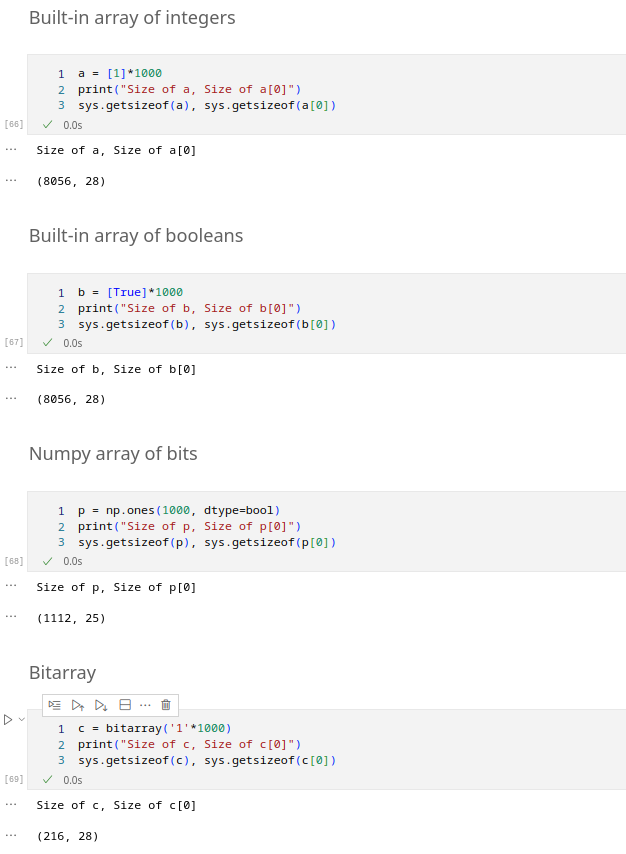
\includegraphics[width=0.5\textwidth]{mem_array.png}
            % \caption{}
            \label{fig:mem_array}
        \end{figure}
\end{frame}

\begin{frame}
        \begin{figure}
            \centering
            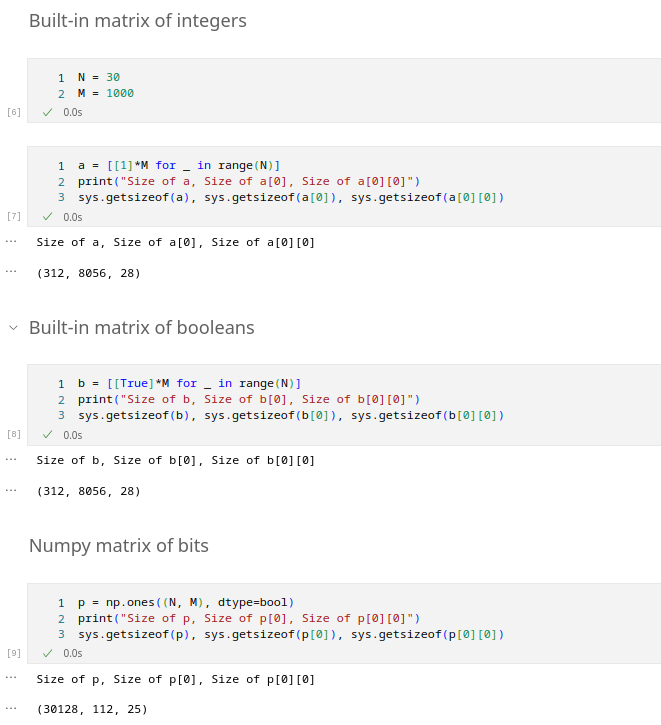
\includegraphics[width=0.55\textwidth]{mem_matrix_1.png}
            \caption{The \texttt{Numpy} matrix requires 30128 bytes to store the raw values of
            the 30000 booleans (around 8.03 bits per boolean).}
            \label{fig:mem_matrix}
        \end{figure}
\end{frame}

% mem_matrix_2
\begin{frame}{}
        % \small
        \begin{figure}
            % \tiny
            \centering
            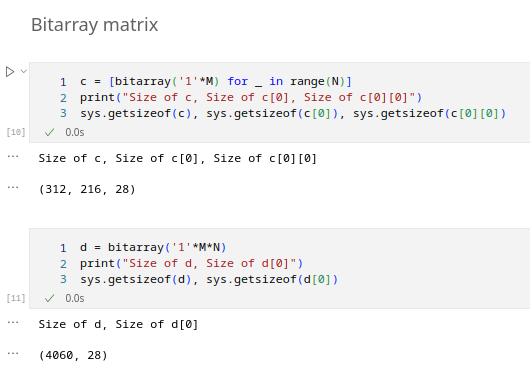
\includegraphics[width=0.55\textwidth]{mem_matrix_2.png}
            \caption{Notice the difference among the two cases. In the first scenario we 
            have a list of bitarrays, although the bitarrays are stored in a contiguous
            block of memory, a different object is dedicated to each bitarray, creating
            an overhead. In the second scenario we have a single bitarray, a single object is
            dedicated to the bitarray, which has the shape of a flattened matrix,
            it occupies 4060 bytes to store 30000 booleans (around 1.082 bits per boolean).
            The second choice is the one I made.}
            \label{fig:mem_matrix_2}
        \end{figure}
\end{frame}

\begin{frame}
    I tried to profile the code with \texttt{memory-profiler} 
    to find whether the memory occupation
    advantages
    I expected to gain from choosing one data structure over the other
    were actually realized, but I could not see any significant difference
    in memory usage while executing the code, I guess this happens because
    the amount of memory required to store the matrices is negligible compared
    to the amount of memory required to store the set of solutions, the set of explored nodes
    and the stack of the recursive calls.
\end{frame}

% \section*{Exploring the solutions}

\begin{frame}{Exploring the solutions}
    % \frametitle{}
    Different cardinalities of the domain (columns of the matrix A) and
    different quantities of sets (rows of the matrix A, rows and columns of the matrix B) 
    lead to different values of:
    \begin{itemize}
        \item the number of solutions found;
        \item the number of explored nodes to find the solutions;
        \item the time required to find the solutions.
    \end{itemize}
    In the following slides I show the values of these quantities for different
    automatically generated instances of the problem. I kept the 
    number of sets in a range between $\sim20$ and $\sim400$ and the cardinality of the domain
    in a range between $\sim5$ and $\sim14$ to contain the duration of the experiments.
\end{frame}

\begin{frame}{Solutions found}
    It is intuitive that the number of solutions found increases
    with the number of sets and decrease with the cardinality of the domain.
    In this case the intuition is confirmed by the solutions found (\ref{fig:sol_5x5}).
\end{frame}

\begin{frame}
    \begin{figure}
        \centering
        \includegraphics[width=0.6\textwidth]{sol_5x5.pdf}
        \caption{The number of solutions found increases with the number of sets 
        and decreases with the cardinality of the domain.}
        \label{fig:sol_5x5}
    \end{figure}
\end{frame}

\begin{frame}{Explored nodes}
    It might seem intuitive that, similarly to the previous case, the number of explored nodes
    increases with the number of sets and decreases with the cardinality of the domain,
    however, the same problems that were solved in the previous case display a different
    and less intuitive behaviour in this case (\ref{fig:explored_5x5}).
    The interpretation of this behaviour is that the algorithm has to work harder,
    that is, to explore more nodes, to find the solutions for more complex problems, that
    is, those problems with a greater number of rows and a greater number of columns.
    Notice that the graphs in figure (\ref{fig:explored_5x5}) follow the same pattern
    as the graphs in figure (\ref{fig:base_star_5x5}) that describes the time required to find all
    the solutions to the same problems.
    Why, fixing the number of rows, the choice of a smaller number of columns leads to a greater
    number of explored nodes? 
\end{frame}    

\begin{frame}{}    
    This behaviour is probably due to the fact that the rows
    of the matrix $A$ were generated by sampling from a uniform distribution the values 
    $\{0, 1\}$ (the slide \textit{Generating Exact Cover problems} explains how 
    the exact cover problems used here were generated), when the number of columns is small, each row is more likely to be 
    compatible with other rows, so it has to be explored more deeply, whereas when the 
    number of columns is greater, given that each row contains around half 1s and half 0s,
    it is more likely that a row is incompatible with other rows, so less rows need to be 
    explored.
    In the slide \textit{More or less 1s} an alternative that
    makes use of different distributions to generate the rows of the matrix $A$ is presented.
\end{frame}

\begin{frame}
    \begin{figure}
        \centering
        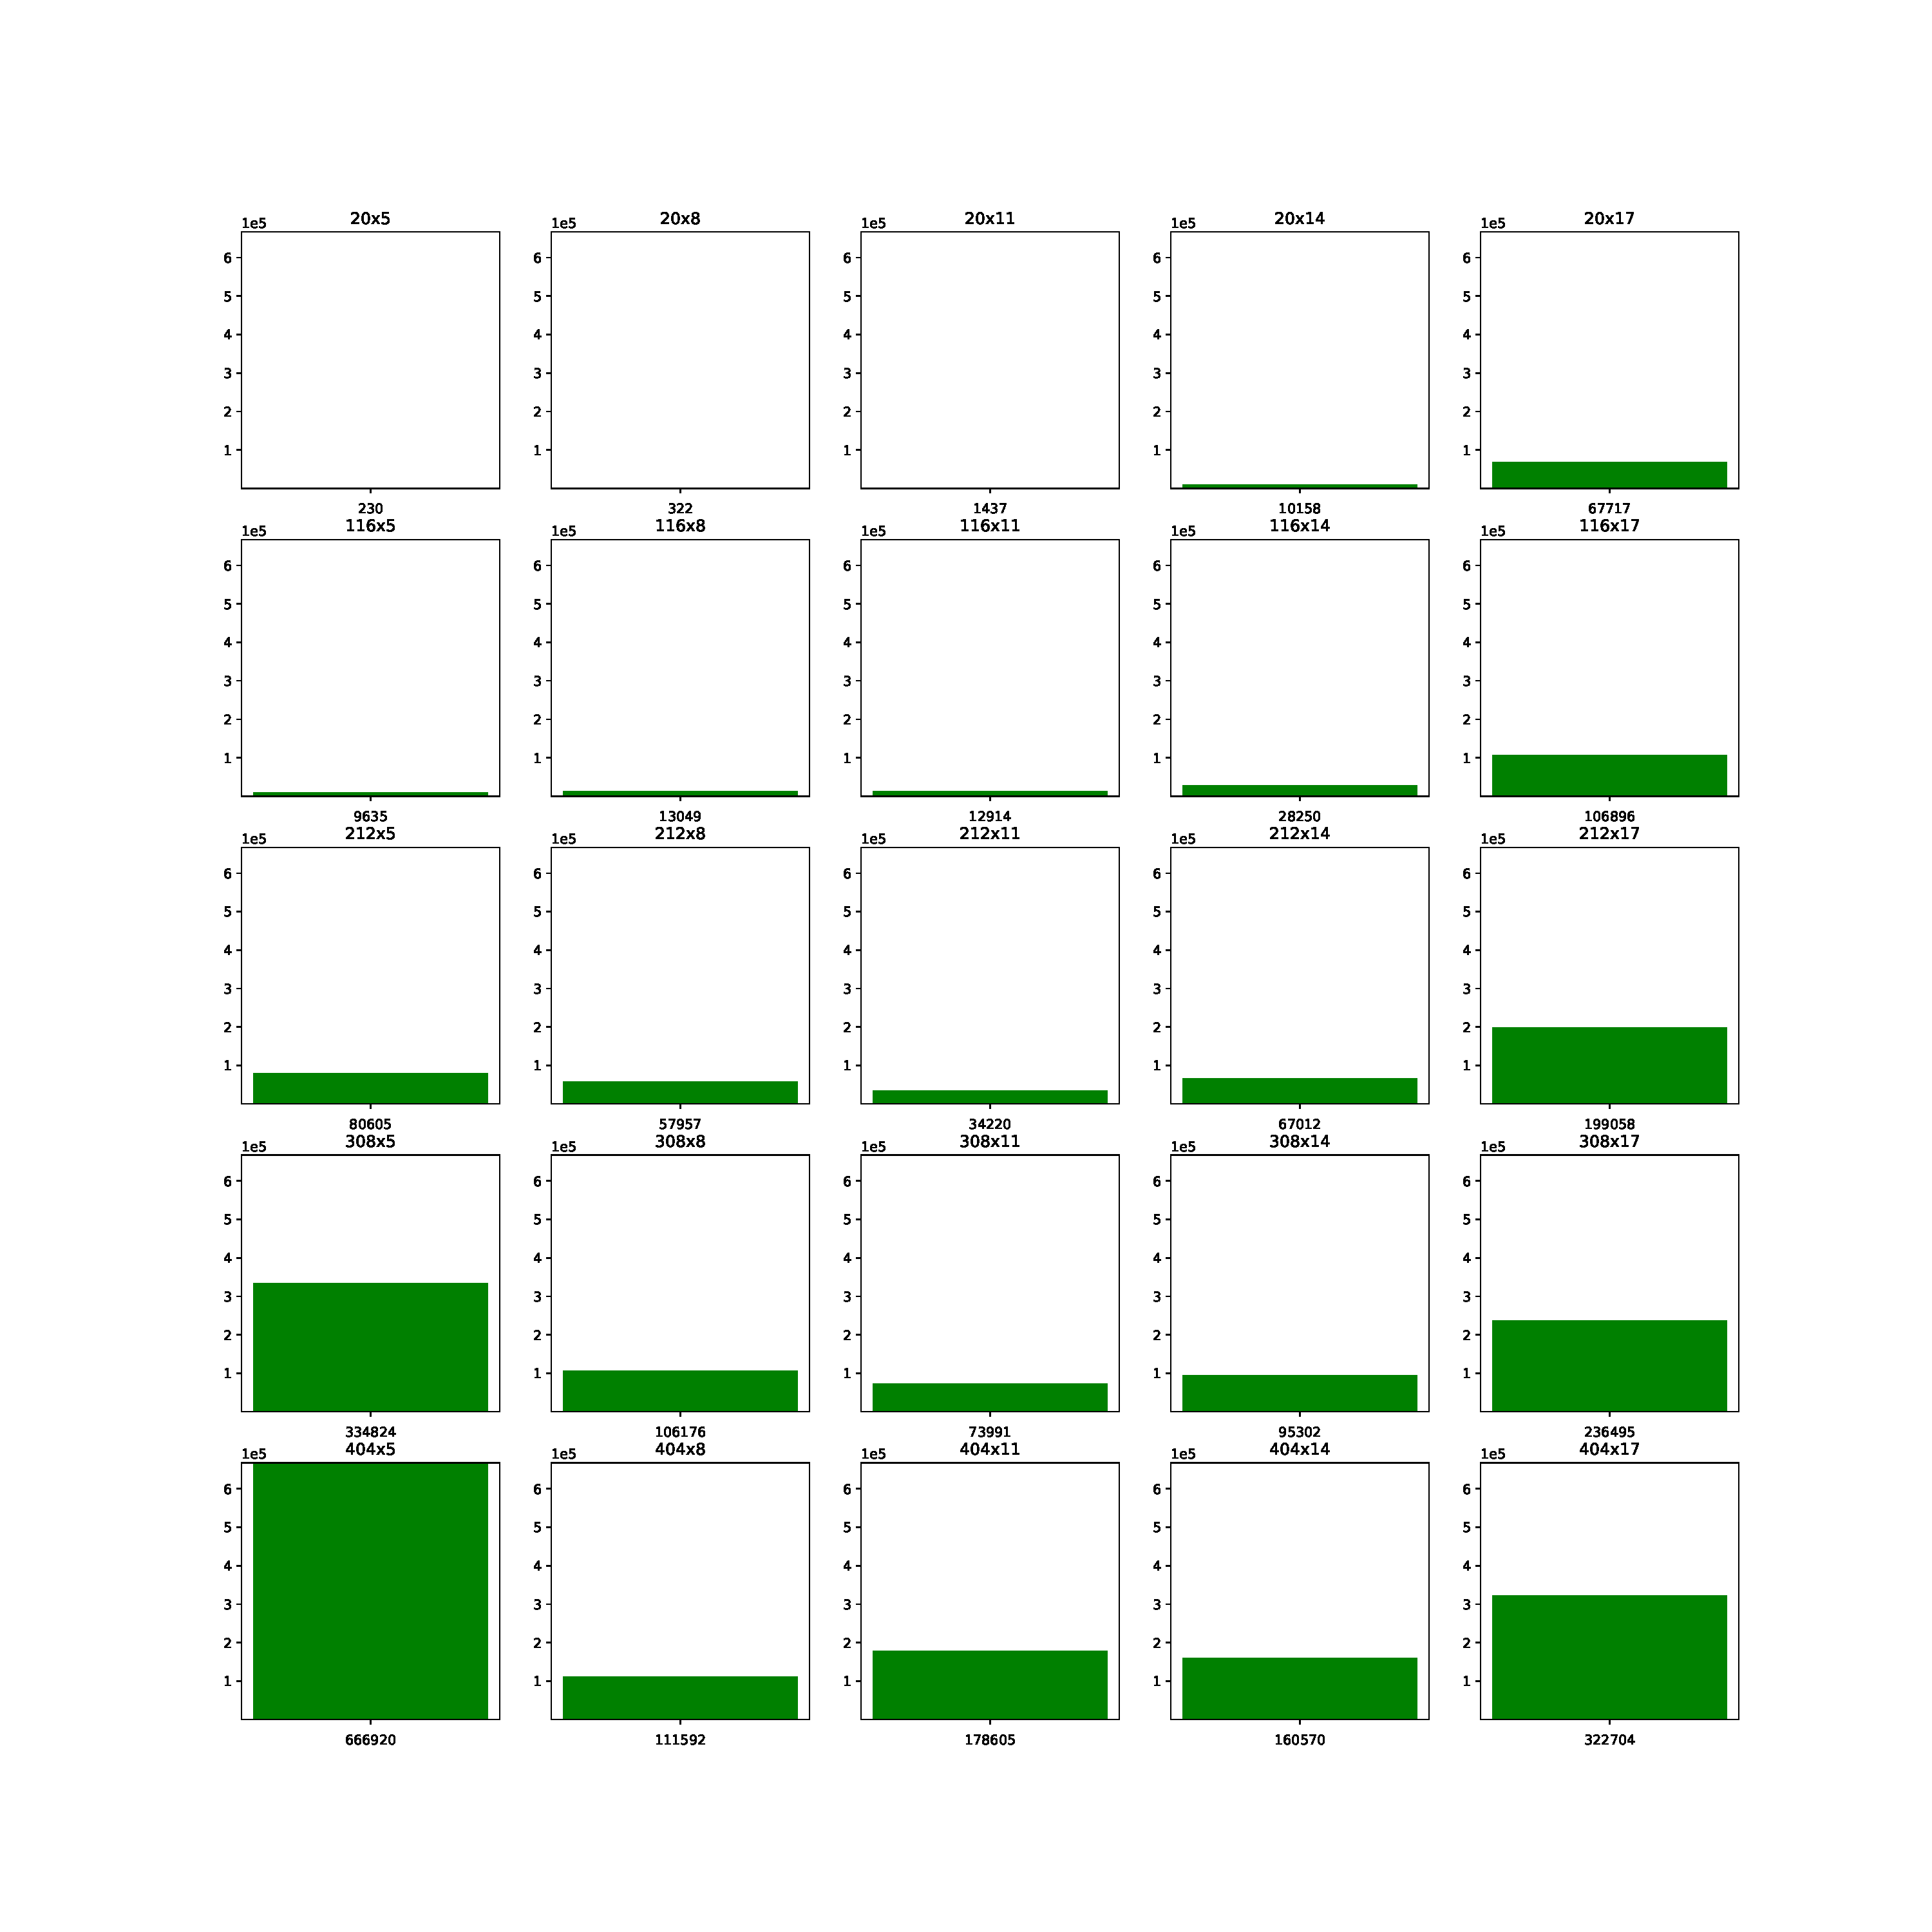
\includegraphics[width=0.5\textwidth]{explored_5x5.pdf}
        \caption{The number of explored nodes increases with the number of sets and increases
        when the cardinality of the domain is too small or too large. The only interpretation
        I could find is that the number of explored nodes increases with the complexity of the problem.}
        \label{fig:explored_5x5}
    \end{figure}
\end{frame}

\begin{frame}{Explorable nodes}
    The implemented algorithm chooses to prune many subtrees
    that will not lead to a plausible solution.
    Professor Marina Zanella showed that if the algorithm blindly decided not to prune any subtree,
    then the number of nodes to explore would be:
    \begin{equation*}
        \sum_{i=1}^{N}\sum_{j=1}^{i}\binom{i}{j} = 2^N-1.
    \end{equation*}

    In figure (\ref{fig:explored_vs_explorable_5x5}) the enormous difference
    between the number of explored nodes and the number of explorable nodes is shown.
\end{frame}

\begin{frame}
    \begin{figure}
        \centering
        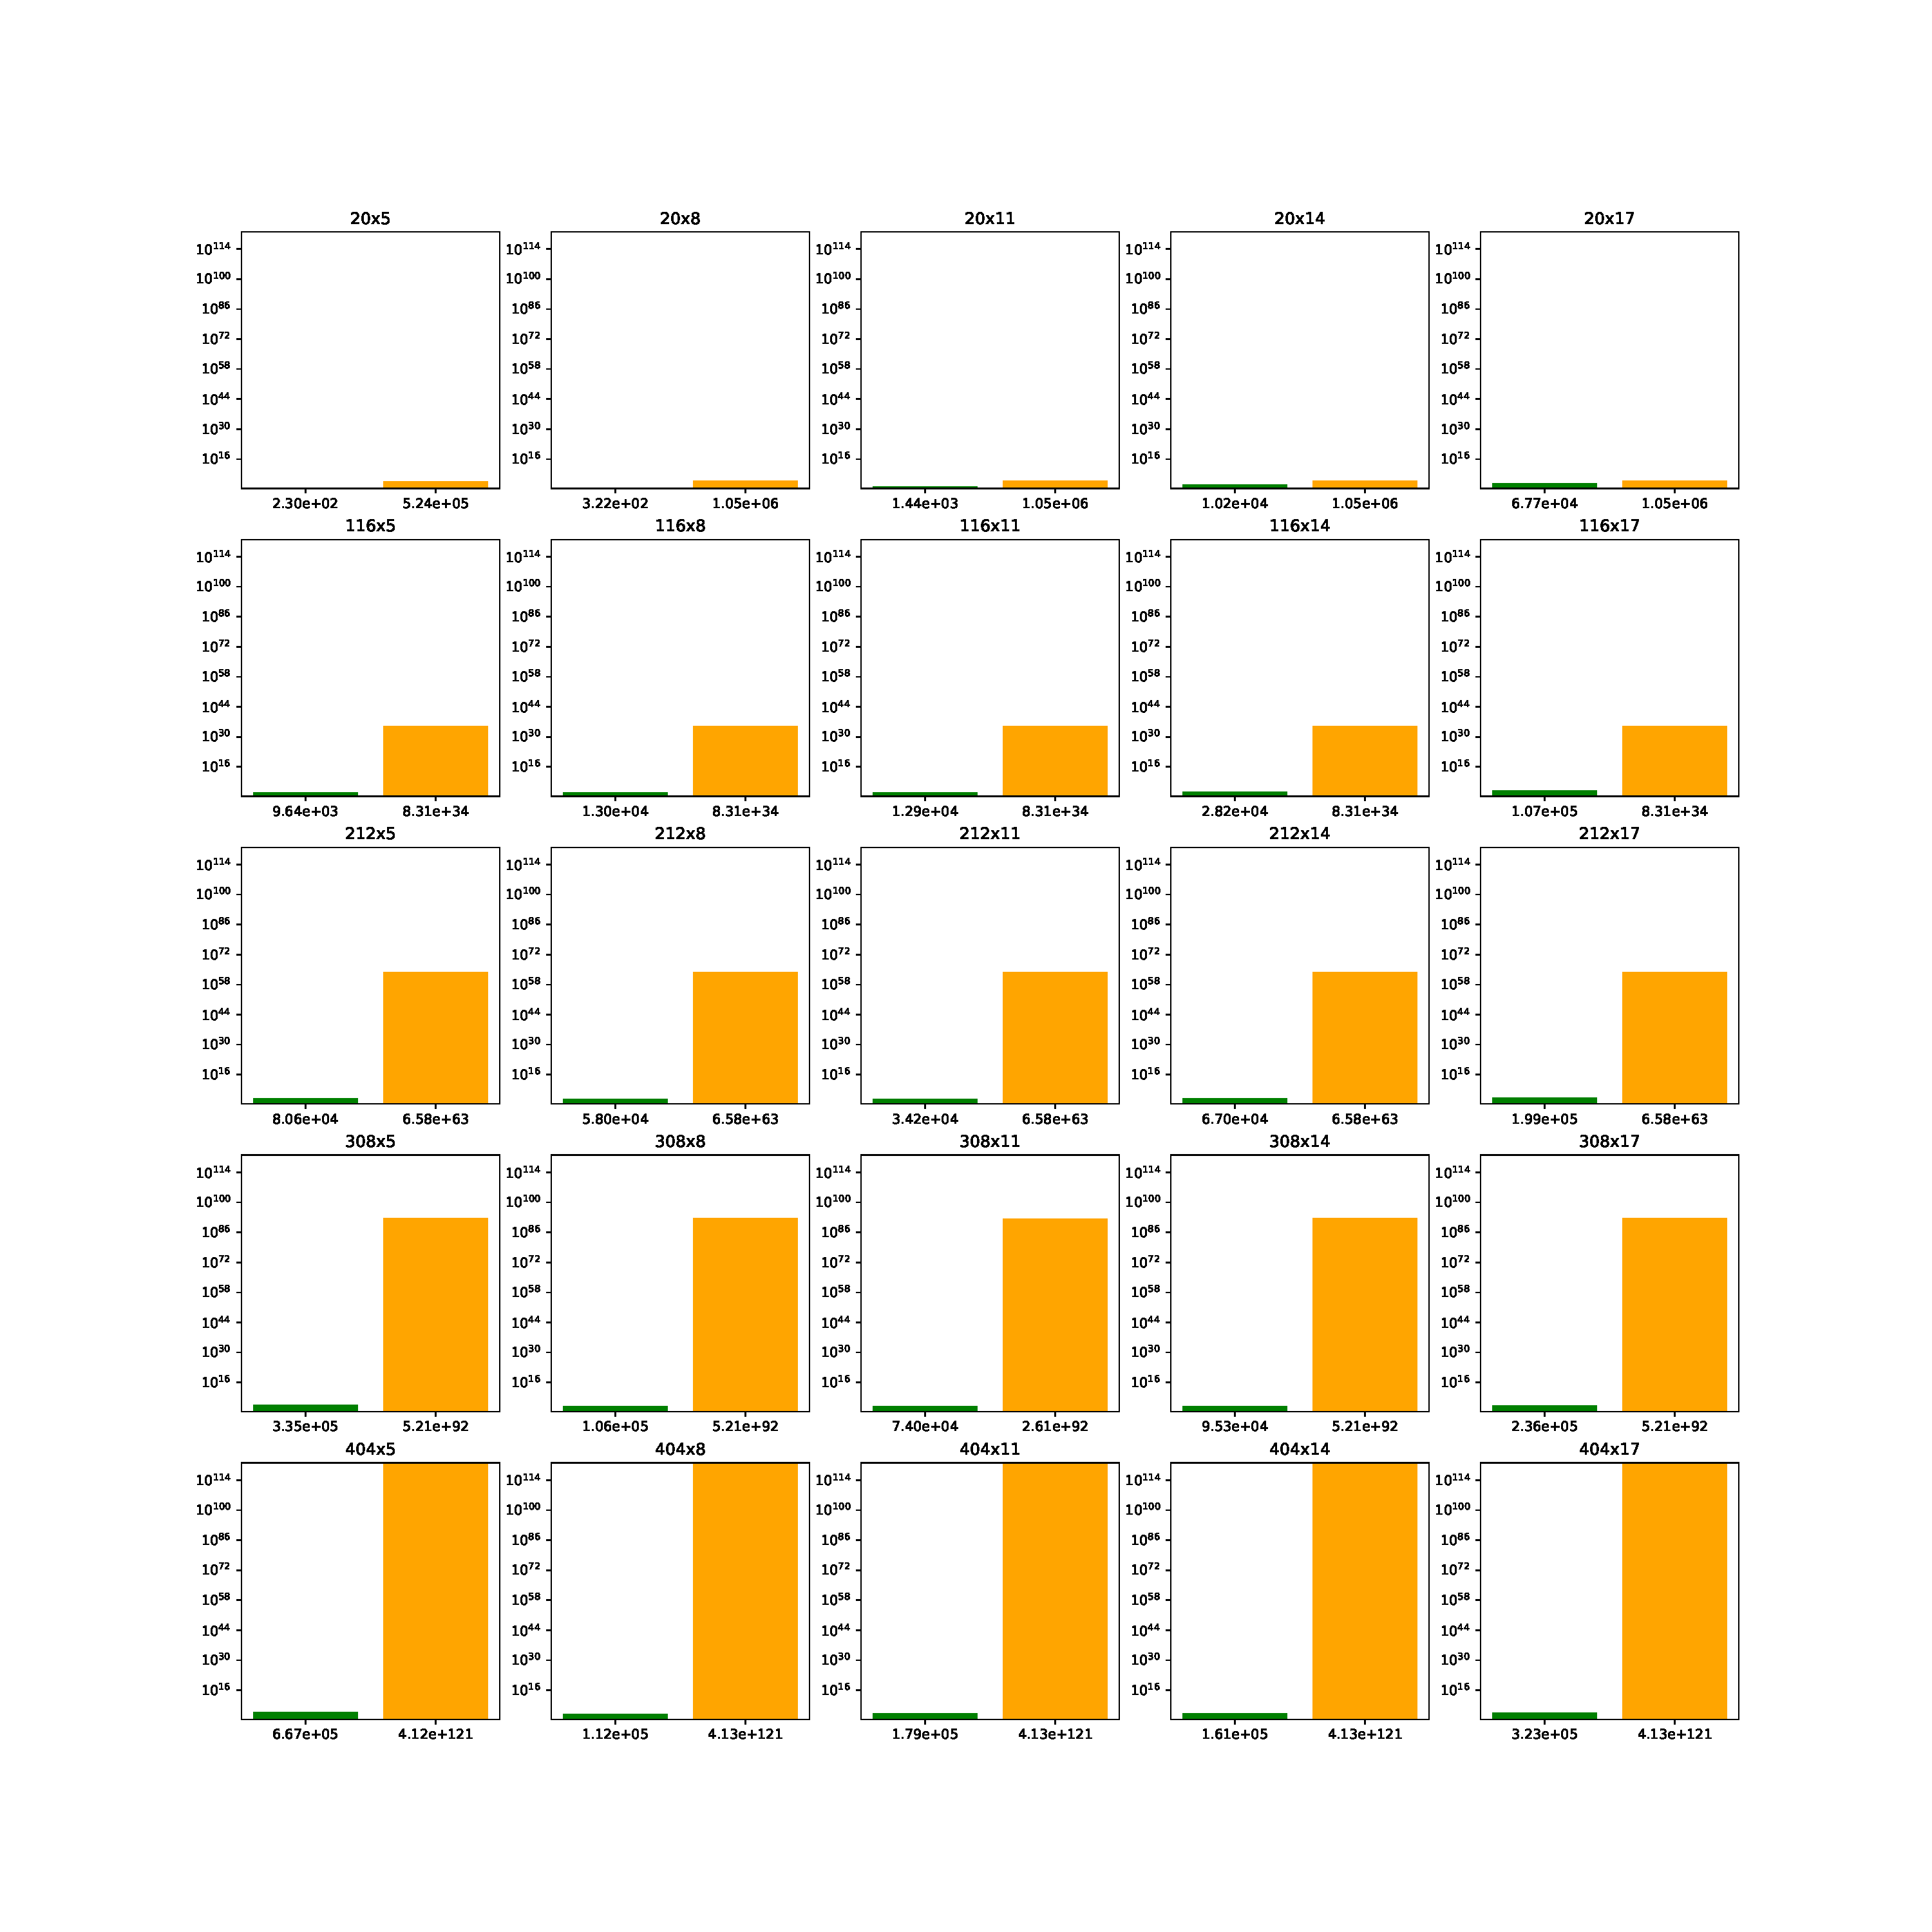
\includegraphics[width=0.5\textwidth]{explored_vs_explorable_5x5.pdf}
        \caption{The number of nodes that would be explored by a blind algorithm is
        much greater than the number of nodes that are actually explored by the implemented algorithm.}
        \label{fig:explored_vs_explorable_5x5}
    \end{figure}
\end{frame}

\begin{frame}{Loading portions}
    The problem to solve might require a huge matrix A,
    to prevent the computer from running out of memory
    one of the possible solutions is to load portions of the matrix
    and solve the problem for each portion, growing incrementally
    the set of solutions (this mechanism is described in the slide \textit{EC wrapper}).
    What is expected is that loading the whole matrix and solving
    at once is faster than loading portions of the matrix.
    The results shown in figure (\ref{fig:loadable_rows_time_diff}), 
    (\ref{fig:loadable_rows_time_diff_rev}) and (\ref{fig:loadable_rows_time_diff_shuffled})
    show something different.
    What can be noticed is that the greatest advantage that comes
    from decreasing the dimension of the chunk of loaded rows is gained
    when it grows from 1 to the second smallest dimension, then there is no clear advantage,
    sometimes loading a greater number of rows at once is faster
    and sometimes it's slower.
    To make the order in which the problems were solved as less influential as possible 
    on the time required, the problems were first solved with an increasing number of loadable rows (figure (\ref{fig:loadable_rows_time_diff})),
    then with a decreasing number of loadable rows (figure (\ref{fig:loadable_rows_time_diff_rev})) and finally with a random number of loadable rows
    (figure (\ref{fig:loadable_rows_time_diff_shuffled})).
\end{frame}

\begin{frame}
    \begin{figure}
        \centering
        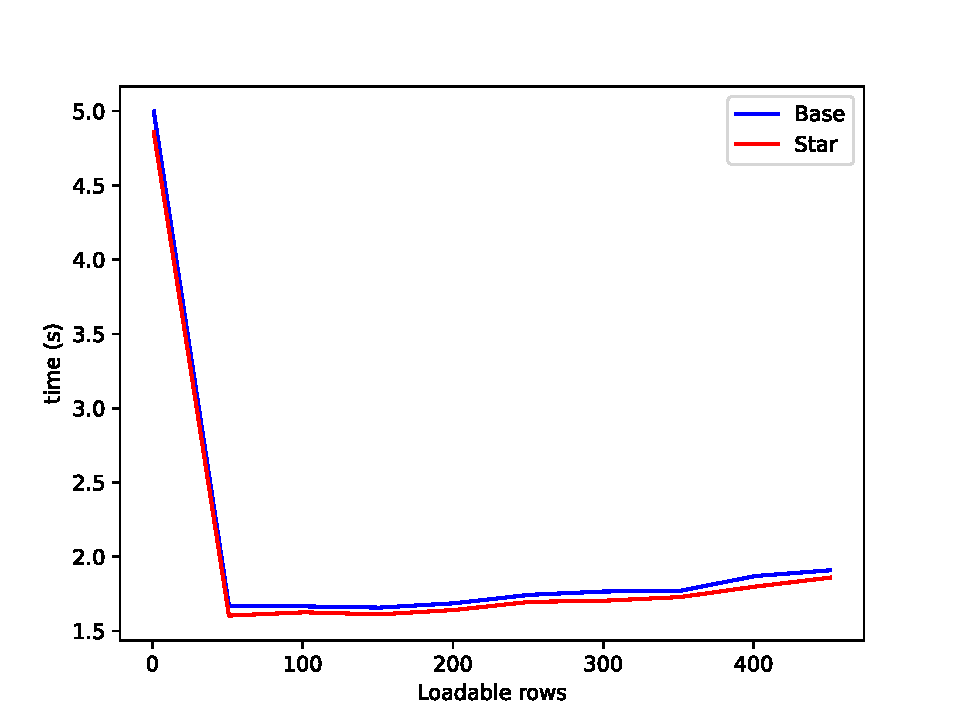
\includegraphics[width=0.75\textwidth]{loadable_rows_time_diff.pdf}
        % \caption{}
        \label{fig:loadable_rows_time_diff}
    \end{figure}
\end{frame}

\begin{frame}
    \begin{figure}
        \centering
        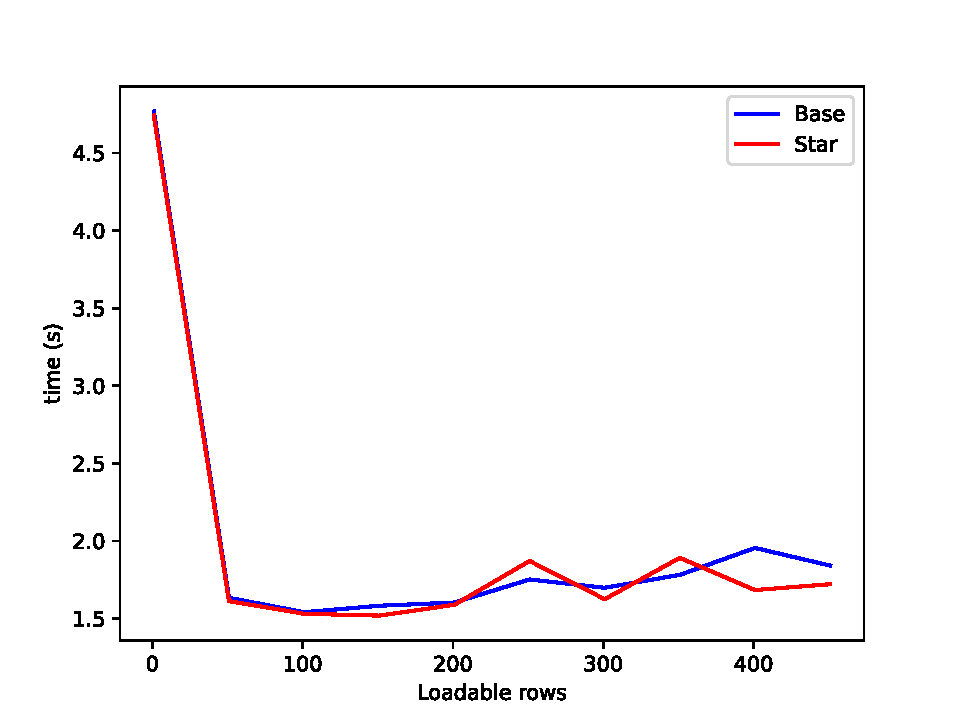
\includegraphics[width=0.75\textwidth]{loadable_rows_time_diff_rev.pdf}
        % \caption{}
        \label{fig:loadable_rows_time_diff_rev}
    \end{figure}
\end{frame}

\begin{frame}{}
    \begin{figure}
        \centering
        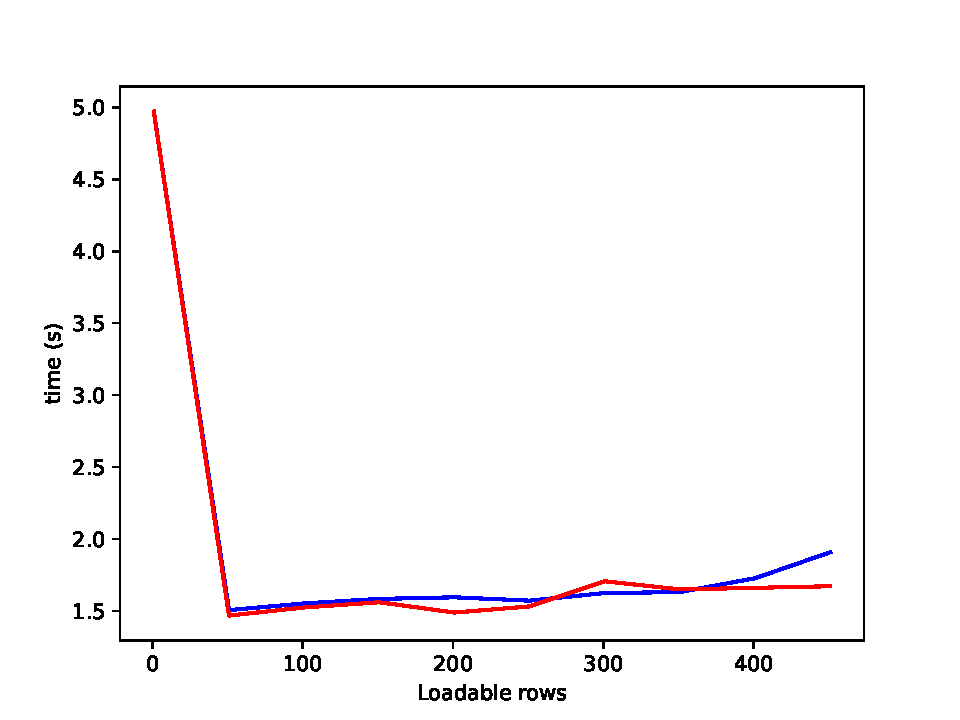
\includegraphics[width=0.75\textwidth]{loadable_rows_time_diff_shuffled.pdf}
        % \caption{}
        \label{fig:loadable_rows_time_diff_shuffled}
    \end{figure}
\end{frame}

\begin{frame}
    A series of manual tests on
    different dimensions of the chunk of loadable rows on a larger problem (1000 rows
    and 15 columns) leaded to the following results:
    % when loading 1 row at a time the algorithm takes 24.5 seconds, 
    % when loading 2 rows it takes 15.3 seconds,
    % when loading 3 rows it takes 12.3 seconds,
    % when loading 5 rows it takes 9.7 seconds, 
    % when loading 10 rows it takes 7.9 seconds,
    % when loading 20 rows it takes 6.9 seconds,
    % when loading 50 rows it takes 6.5 seconds,
    % when loading 100 rows it takes 6.5 seconds,
    % when loading 400 rows it takes 6.6 seconds.
    \begin{itemize}
        \item when loading 1 row at a time the algorithm takes 24.5 seconds;
        \item when loading 2 rows it takes 15.3 seconds;
        \item when loading 3 rows it takes 12.3 seconds;
        \item when loading 5 rows it takes 9.7 seconds;
        \item when loading 10 rows it takes 7.9 seconds;
        \item when loading 20 rows it takes 6.9 seconds;
        \item when loading 50 rows it takes 6.5 seconds;
        \item when loading 100 rows it takes 6.5 seconds;
        \item when loading 400 rows it takes 6.6 seconds;
        \item when loading 900 rows it takes 7.1 seconds.
        \item when loading 1000 rows it takes 7.6 seconds
    \end{itemize}
    \end{frame}

\begin{frame}{\textit{Base} and \textit{plus} algorithms}
    The previous experiments leaded also to the conclusion that the \textit{plus} algorithm, most of the times,
    is slightly faster than the \textit{base} algorithm, but it remains unclear
    why sometimes this is not the case.
    The same unpredictable behaviour is shown in figure (\ref{fig:base_star_5x5}).
\end{frame}

\begin{frame}{}
    \begin{figure}
        \centering
        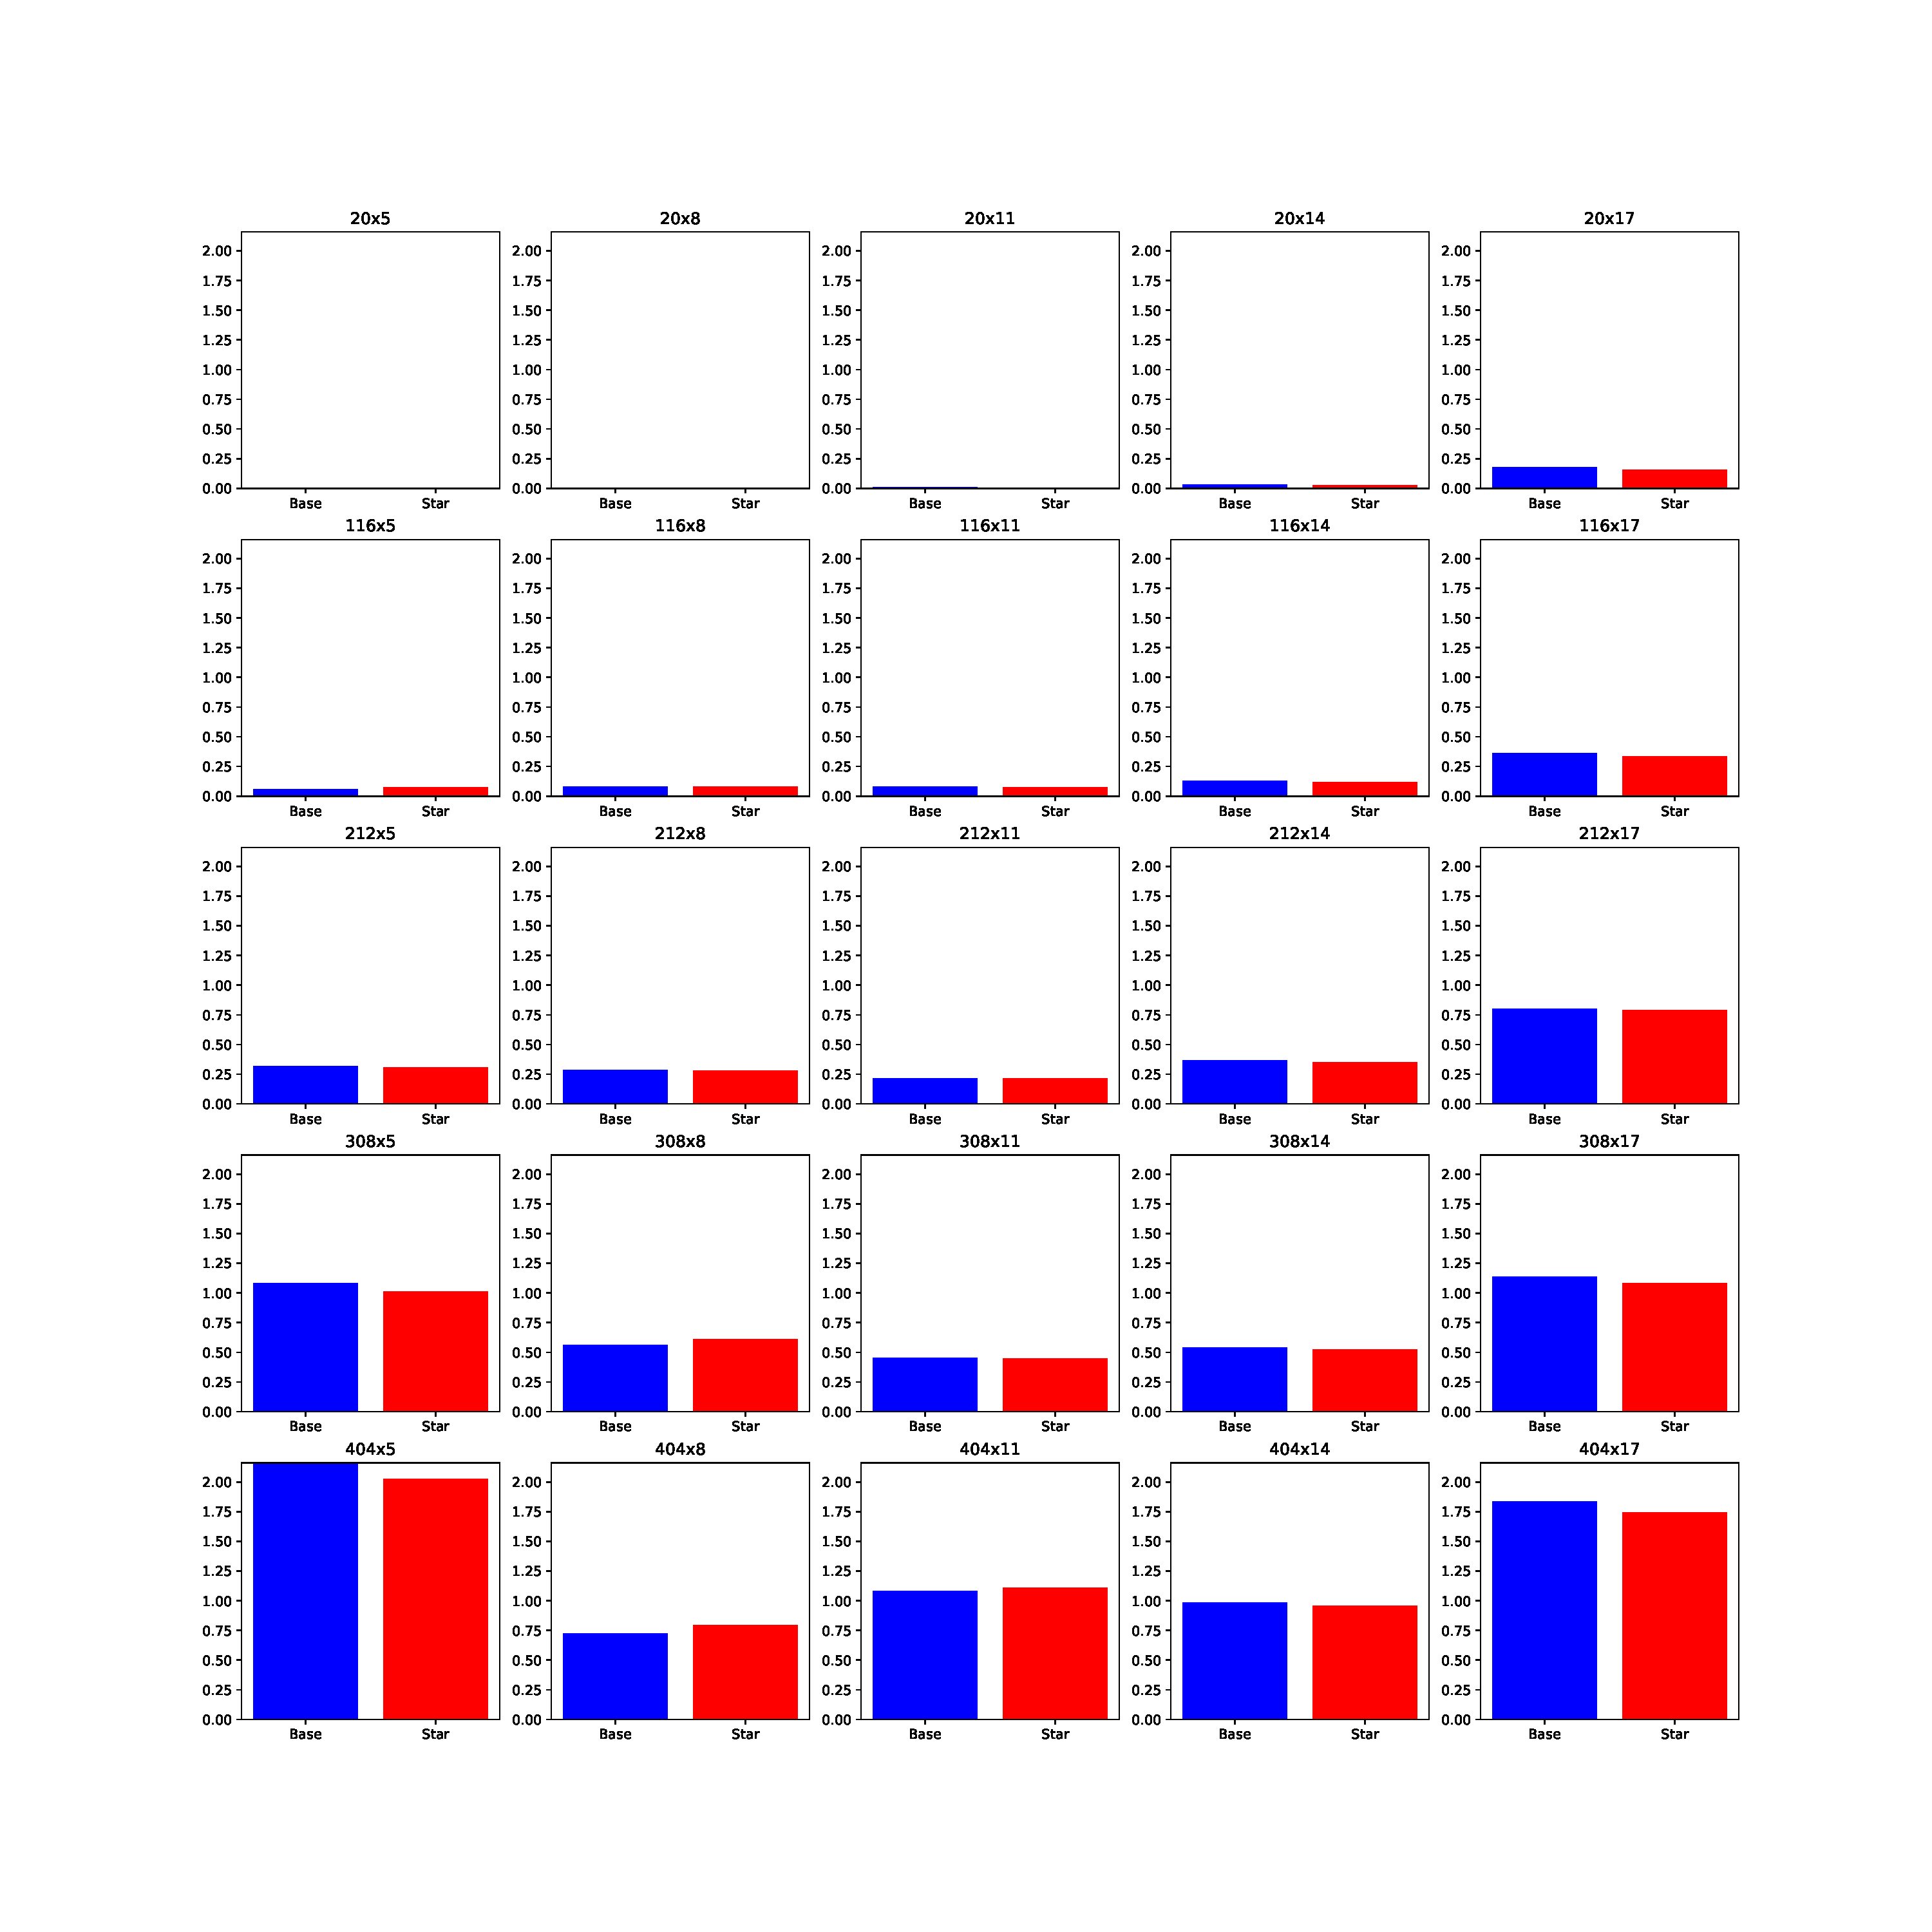
\includegraphics[width=0.5\textwidth]{base_star_5x5.pdf}
        \caption{This figure shows the time required to find all the solutions to the same problems
        whose results were shown before, in particular, the graph shows the same pattern as in figure (\ref{fig:explored_5x5}).
        The \textit{plus} algorithm is slightly faster than the \textit{base} algorithm, but it remains unclear
        why sometimes this is not the case.}
        \label{fig:base_star_5x5}
    \end{figure}
\end{frame}

\begin{frame}{More or less 1s}
    For a better comprehension of how the number of explored nodes 
    depends on the structure of the problem, one possibility
    is to generate random exact cover problems varying the sparsity
    of the matrix $A$.
    The intuition is that the more 1s there are in each row
    of the matrix $A$, the more difficult it is for the problem
    to have different rows that are compatible,
    hence, the more difficult it is for the algorithm to find
     solutions and the more nodes it has to explore.
    The more 0s there are in each row of the matrix $A$, the more
    likely it is for the problem to find the solutions,
    each partition (solution) will contain more sets (rows) since each row contains
    fewer 1s, hence, the algorithm will encounter less obstacles
    in finding the solutions and will prune less branches (so it will explore
    more nodes).
    The figures (\ref{fig:explored_nodes_prob}), (\ref{fig:solutions_prob})
    and (\ref{fig:time_to_solve_prob}) show the results of the experiments
    and, the larger the number of columns,
    the more our intuition is confirmed.
\end{frame}

\begin{frame}{}
    \begin{figure}
        \centering
        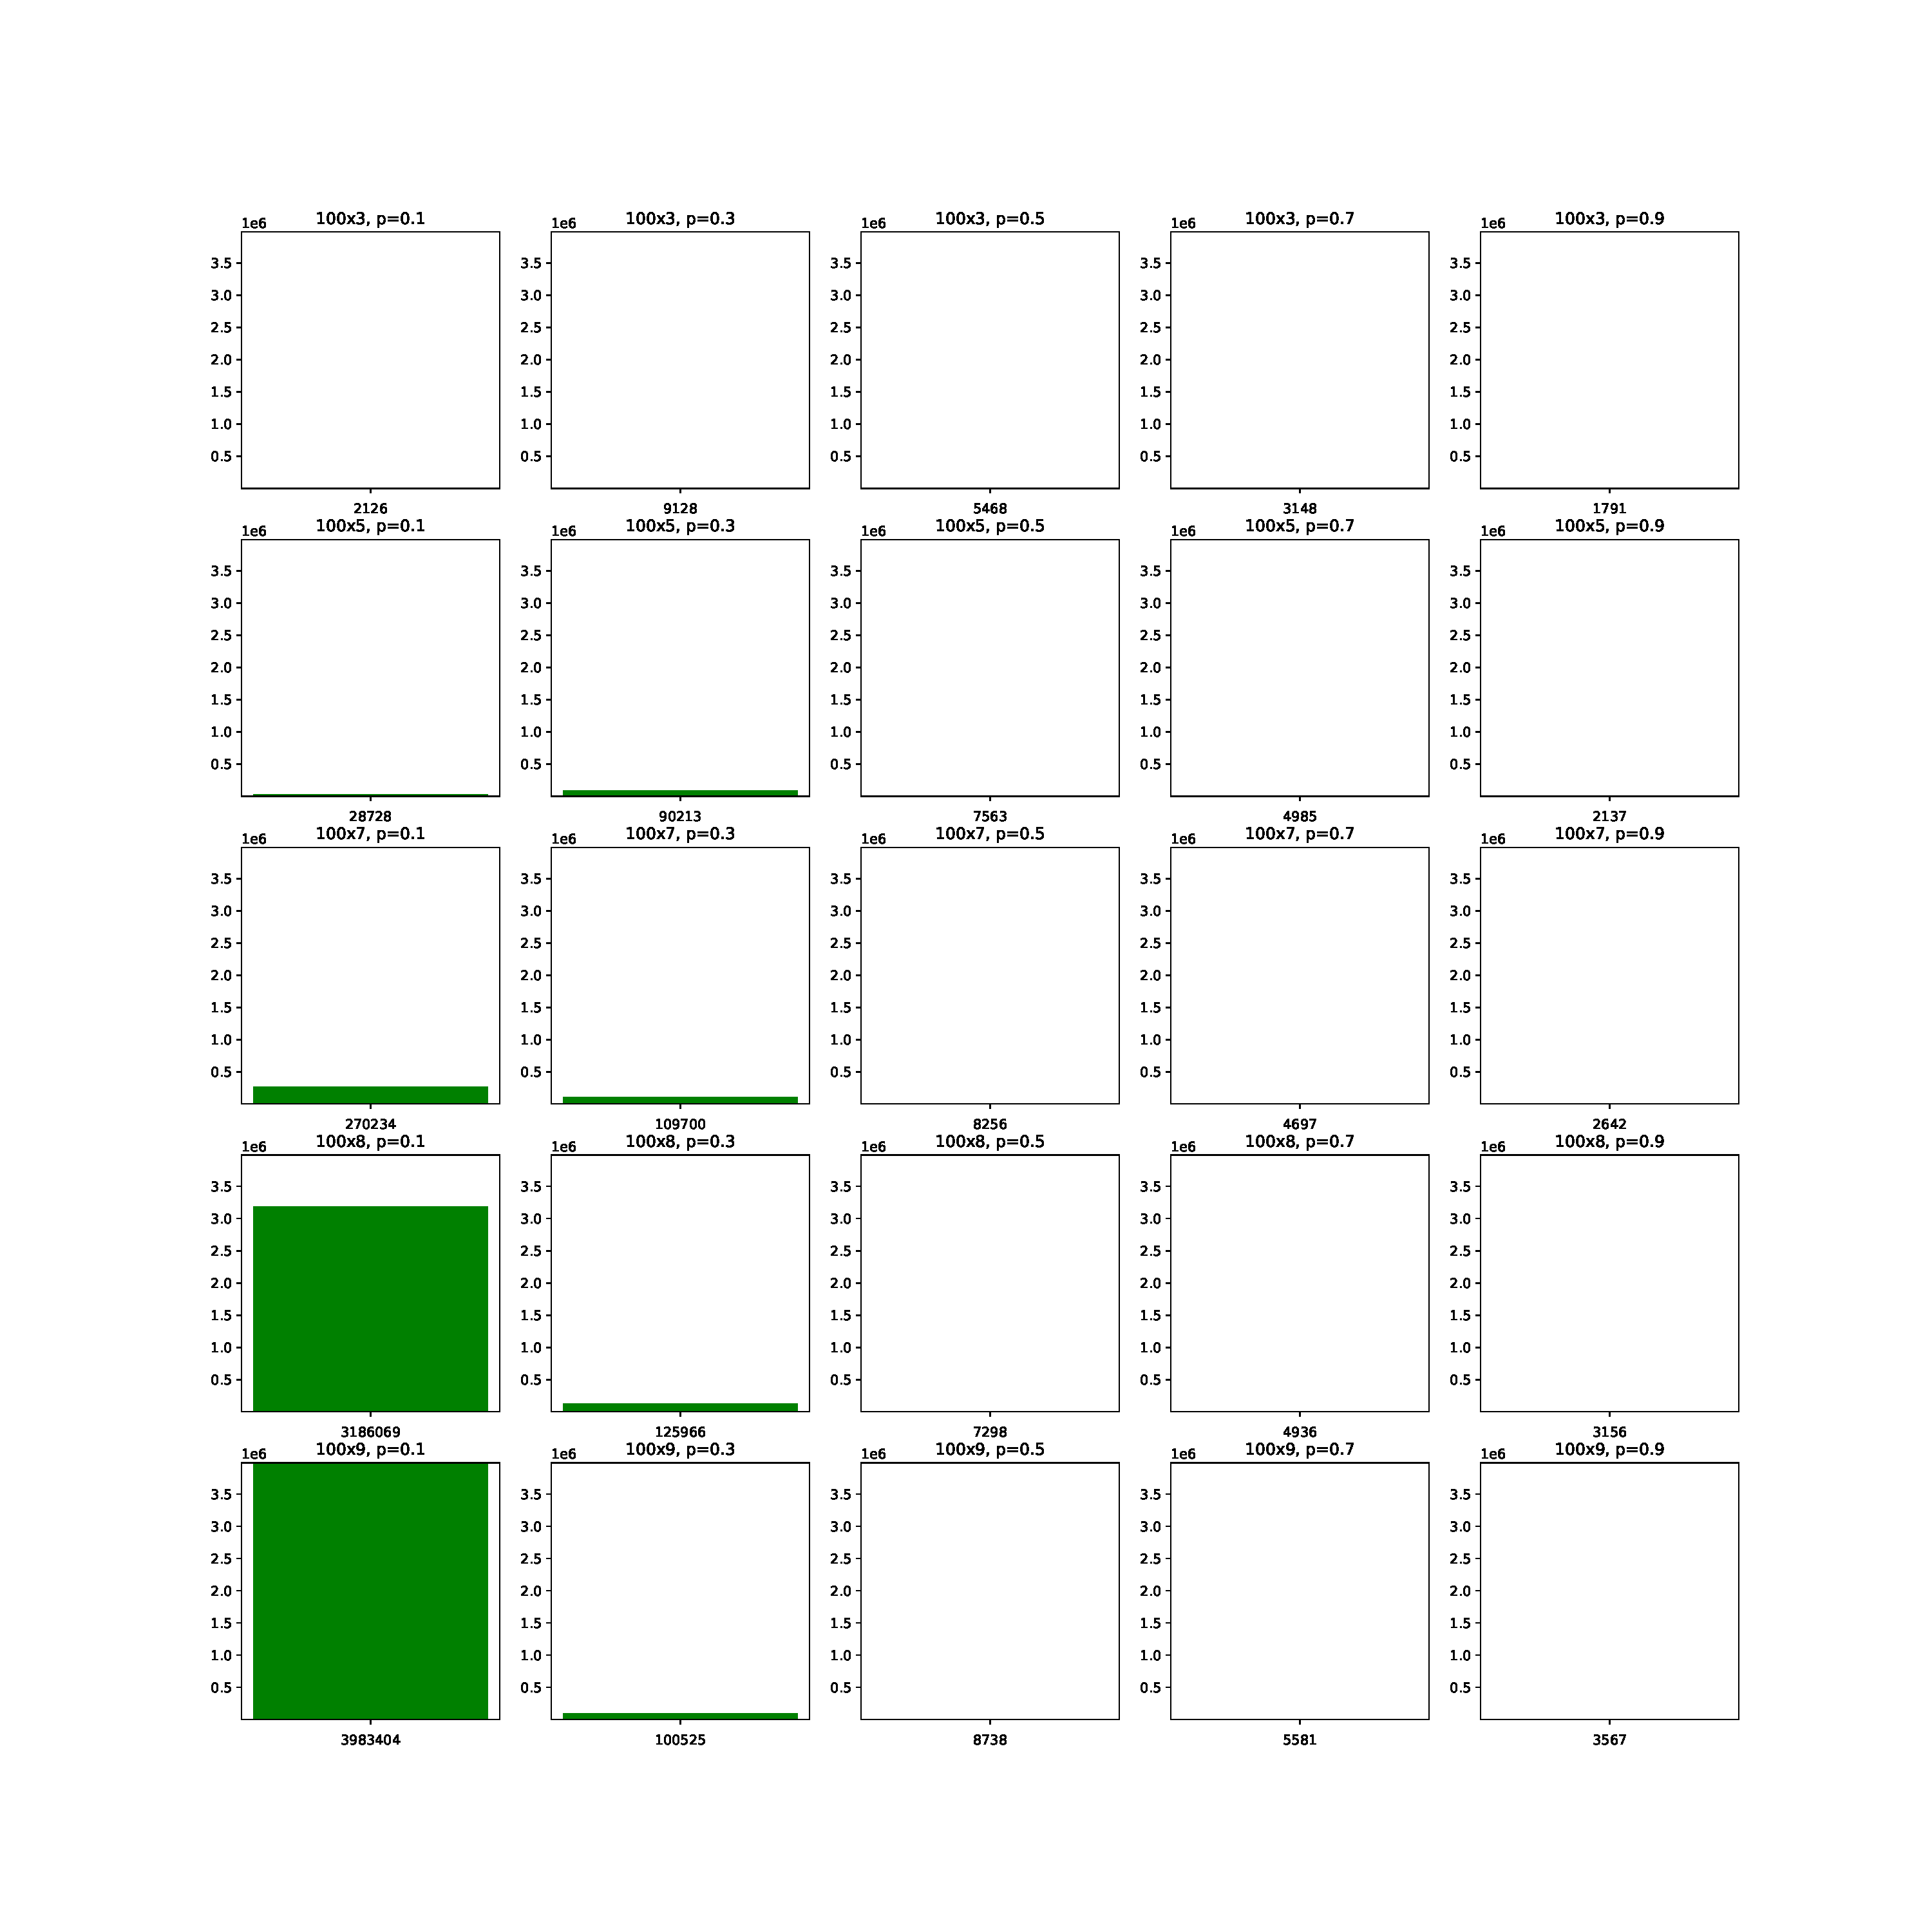
\includegraphics[width=0.5\textwidth]{explored_nodes_prob.pdf}
        \caption{The number of explored nodes increases with the number of rows and 
        decreases with the number of 1s in each row, this is because the more 1s there are,
        the less likely it is for the problem to have compatible rows, hence, the less sets 
        are to be explored, the more 0s there are, the more likely it is for the problem
        to have compatible rows, hence, the more sets are to be explored.}
        \label{fig:explored_nodes_prob}
    \end{figure}
\end{frame}

\begin{frame}{}
    \begin{figure}
        \centering
        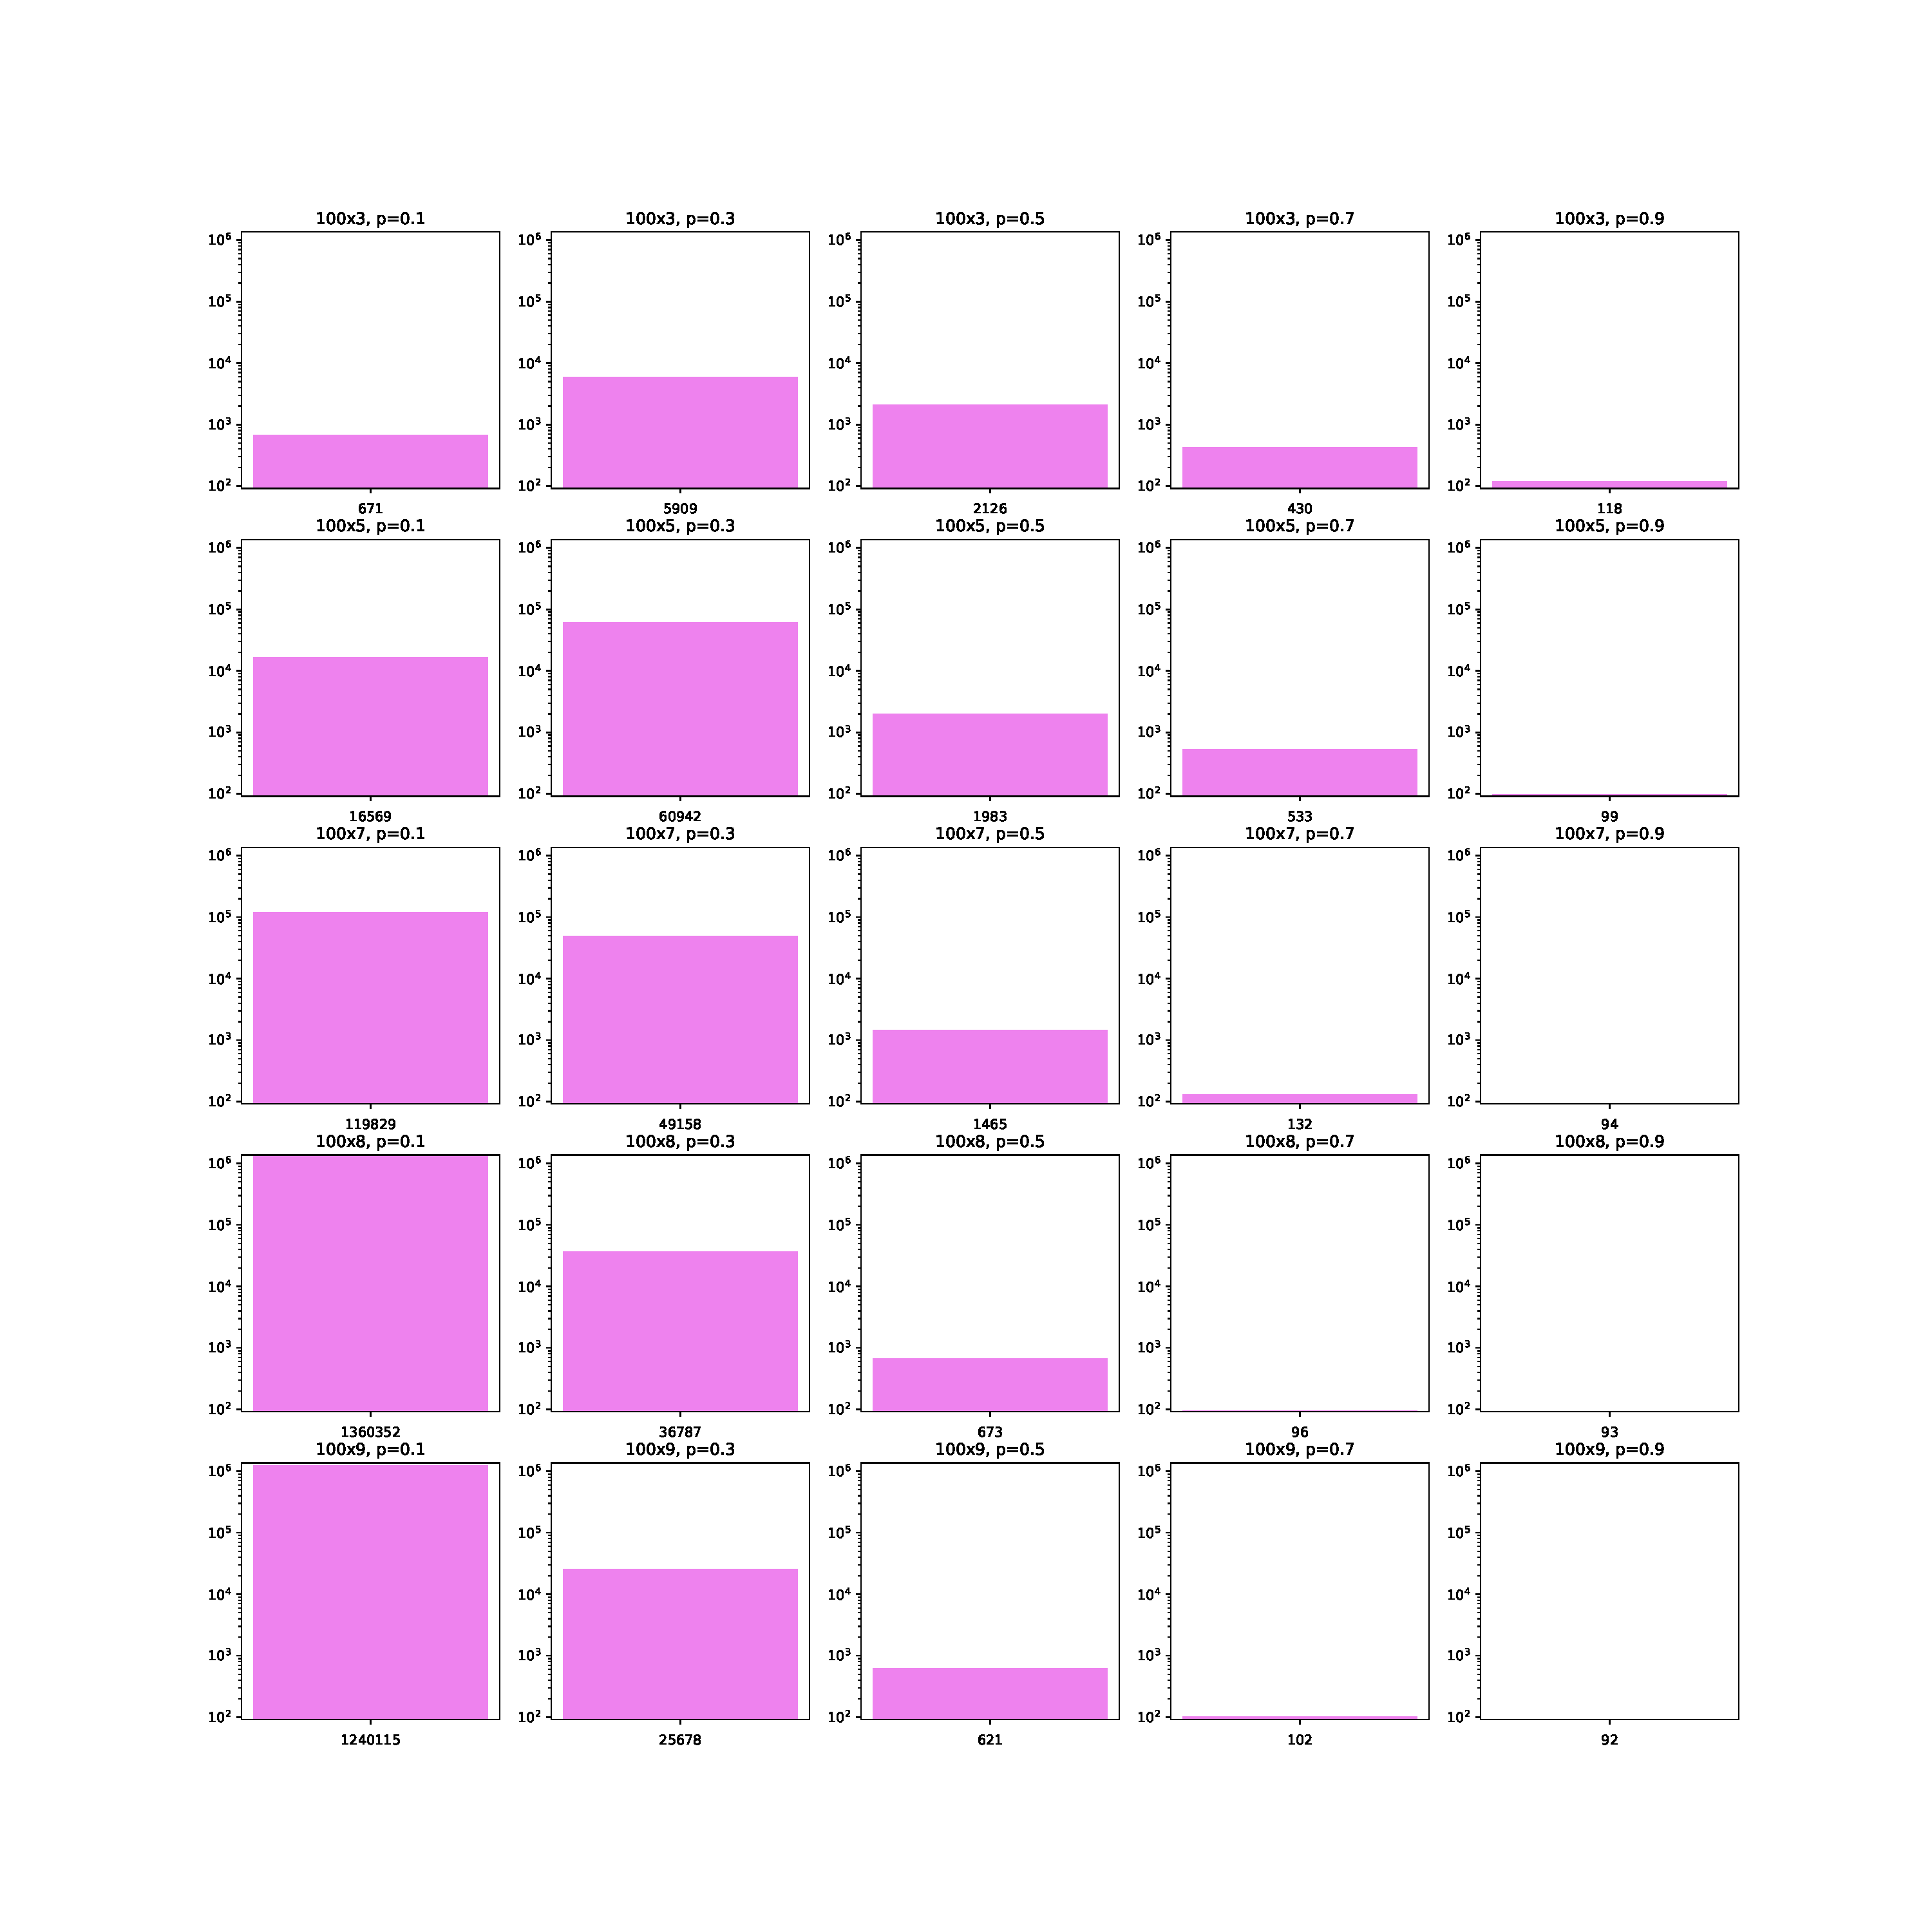
\includegraphics[width=0.5\textwidth]{solutions_prob.pdf}
        \caption{Once the problem has enough columns, the number of solutions found 
        increases with the number of 0s in each row, the reason is the same as before (
        figure (\ref{fig:explored_nodes_prob})).}
        \label{fig:solutions_prob}
    \end{figure}
\end{frame}

\begin{frame}{}
    \begin{figure}
        \centering
        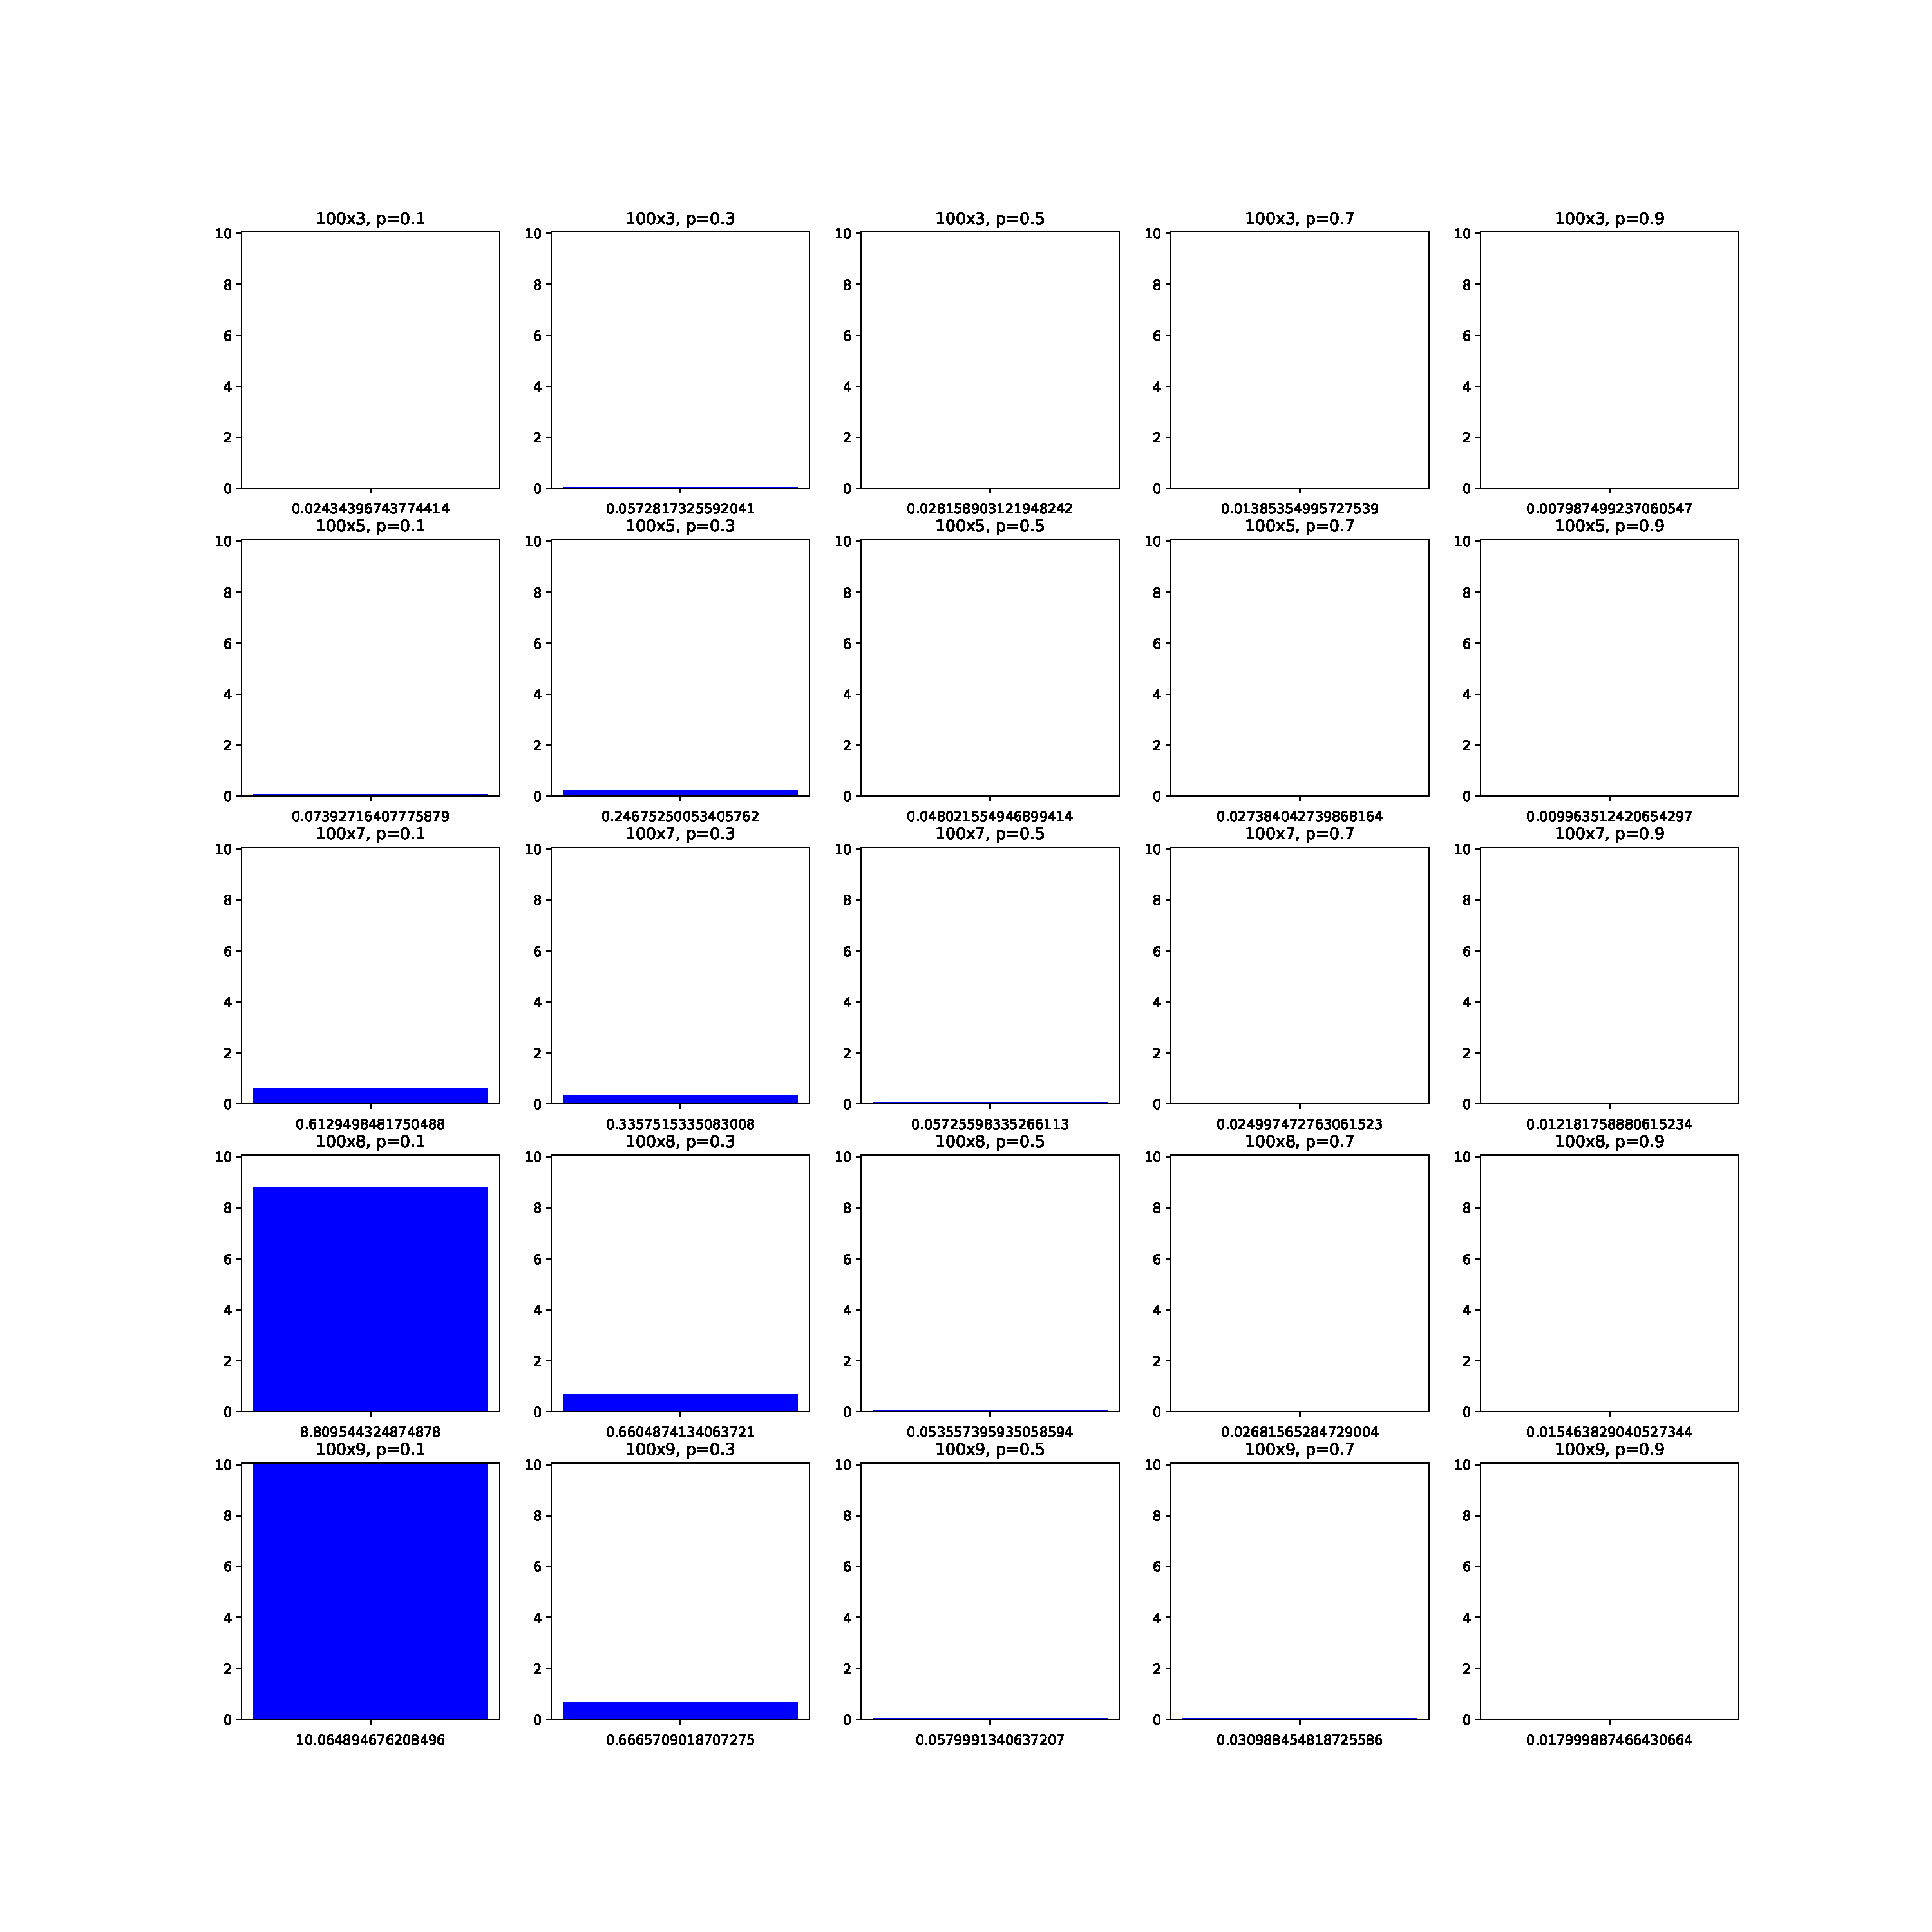
\includegraphics[width=0.5\textwidth]{time_to_solve_prob.pdf}
        \caption{Again, the time required to find the solutions follows the same pattern as 
        the number of explored nodes, shown in figure (\ref{fig:explored_nodes_prob}).}
        \label{fig:time_to_solve_prob}
    \end{figure}
\end{frame}

\begin{frame}{EC wrapper}
    In the following slides the mechanism wrapping the EC algorithm
    is presented. 
    The idea is to load a portion of the matrix A, execute the EC algorithm
    and store the solutions found in a set, then load the next portion of
    the matrix A, execute the EC algorithm and grow the set of solutions.
    The important thing to keep in mind is that when the algorithm 
    is running on a portion of the matrix A, say from row $i$ to row $j$,
    the rows from $0$ to $i-1$ are not immediately available, they need to
    be read from within the EC algorithm, again in portions.
    % color for offset -> #FF1A1A
    % color for reading offset -> #1A40FF
    This explains the need for two variables:
    \textcolor{offset}{offset} and \textcolor{reading_offset}{reading offset}
    (the same colors will be used in the schema and the animation to follow.)
\end{frame}

\begin{frame}{}
    \begin{itemize}
        \item \textcolor{offset}{offset} is the index of the first row of the portion
            of the matrix A that has been passed to the EC algorithm from outside
        \item \textcolor{reading_offset}{reading offset} is the index of the first row of the portion
            of the matrix A that is being read by the EC algorithm,
            reading offset will always start from 0 and will be incremented until
            the rows are read from 0 to the last row of the portion of the matrix A 
            that has been passed to the EC algorithm from outside.
    \end{itemize}
\end{frame}

\begin{frame}{}
    \begin{algorithmic}
        % \Function{CalculateFactorial}{$n$}
        %     \If {$n \leq 1$}
        %         \State \Return 1
        %     \Else
        %         \State $result \gets 1$
        %         \For{$i \gets 1$ to $n$}
        %             \State $result \gets result \times i$
        %         \EndFor
        %         \State \Return $result$
        %     \EndIf
        % \EndFunction
        % \State $x \gets 5$
        % \State $y \gets \Call{CalculateFactorial}{x}$
        % \State \textbf{print} $y$
        \Function{IncrementalExactCover}{$filename$}
            \State $rows \gets \Call{GetRows}{filename}$
            \State $columns \gets \Call{GetColumns}{filename}$
            \State $B \gets \Call{zeros}{rows, columns}$
            \State $COV \gets \Call{set}{\emptyset}$
            \State $offset \gets 0$
            \While{true}
                \State $A \gets \Call{GetPortionOfA}{filename, offset, loadableRows}$
                % If A is empty, break
                \If{$A$ is empty}
                    \State \textbf{break}
                \EndIf
                \State \Call{EC}{$A$, $B$, $COV$, $offset$, $filename$, $loadableRows$}
            \EndWhile
            \State \Return $COV$
        \EndFunction
    \end{algorithmic}
\end{frame}

% \begin{frame}{}
%     \begin{algorithmic}[1]
%         \Function{IncrementalProcess}{$A$, $B$, $COV$, $offset$, $filename$, $loadable\_rows$}
%             \State $new\_COV$ = \Call{EC}{$A$, $B$, $offset$, $filename$, $loadable\_rows$}
%             \State $COV \gets COV \cup new\_COV$
%         \EndFunction
%     \end{algorithmic}
% \end{frame}


\begin{frame}{}
    \scriptsize
    \begin{algorithmic}
        \Function{EC}{$A$, $B$, $COV$, $offset$, $filename$, $loadableRows$}
            \State $N \gets \Call{rows}{A}$ \Comment{Number of rows of A}
            \State $M \gets \Call{columns}{A}$ \Comment{Number of columns of A}
            \For {$i \gets 0$ to $N-1$}
                % row = A[i]
                \State $row \gets A[i]$     
                \If {$\Call{sum}{row} = 0$} \Comment{If the row is all 0s}
                    \For {$t \gets 0$ to $N-1$} \Comment{set the relative
                    row and column of B to 0}
                        \State $B[t][i+offset] \gets 0$
                        \State $B[i+offset][t] \gets 0$
                    \EndFor
                    \State \textbf{continue}  
                \EndIf  
                    
                    % if sum(row_data) == M:
                    % for t in range(N):
                    %     B[t][i+offset] = 0
                    %     B[i+offset][t] = 0
                    % COV.add((offset + i,))
                    % continue    
                \If {$\Call{sum}{row} = M$} \Comment{If the row is all 1s}
                    \For {$t \gets 0$ to $N-1$} \Comment{set the relative
                    row and column of B to 0}
                        \State $B[t][i+offset] \gets 0$
                        \State $B[i+offset][t] \gets 0$
                    \EndFor
                    \State $COV \gets COV \cup \{(offset + i,)\}$
                    \State \textbf{continue}
                \EndIf

                \State $readingOffset \gets 0$

                \State \Call{WhileCycle}{$A$, $B$, $COV$, $offset$, $filename$, $loadableRows$, $i$, $readingOffset$}
            \EndFor
        \EndFunction
    \end{algorithmic}
\end{frame}

\begin{frame}{}
    \tiny
    \begin{algorithmic}
        \Function{WhileCycle}{$A$, $B$, $COV$, $offset$, $filename$, $loadableRows$, $i$, $readingOffset$}

            \While{$readingOffset < i + offset$}
                \State $oldA \gets \Call{GetPortionOfA}{filename, readingOffset, loadableRows}$

                % \State $j \gets 0$ to $\Call{min}{\Call{rows}{oldA}, i + offset - readingOffset} - 1$
                \State $numRows \gets \Call{rows}{oldA}$
                \State $endVal \gets \Call{min}{numRows, i + offset - readingOffset} - 1$
                \For {$j \gets 0$ to $endVal$}
                    \State $oldRow \gets oldA[j]$

                    \If {$\Call{sum}{oldRow} \in \{0, M\}$}
                        \State \textbf{continue}
                    \EndIf
                    
                    \If {$\Call{intersect}{oldRow, row}$}
                        \State $B[j + readingOffset][i + offset] \gets 0$
                    \Else
                        \State $I \gets (offset + i, j + readingOffset)$
                        \State $U \gets \Call{union}{oldRow, row}$
                        \If {$\Call{sum}{U} = M$}
                            \State $COV \gets COV \cup \{I\}$
                            \State $B[j + readingOffset][i + offset] \gets 0$
                        \Else
                            \State $B[j + readingOffset][i + offset] \gets 1$
                            % \State $intersect \gets \{k \mid k \in \{0, \dots, j + readingOffset - 1\} \text{ and } B[k][i + offset] \text{ and } B[k][j + readingOffset]\}$
                            \State $intersect \gets []$ % \Comment{intersect is the set of indices of rows of A that have a 1 in both columns $i + offset$ and $j + readingOffset$}
                            \For {$k \gets 0$ to $j + readingOffset - 1$}
                                \If {$B[k][i + offset] = 1 \text{ and } B[k][j + readingOffset] = 1$}
                                    % \State $intersect \gets intersect \cup \{k\}$
                                    \State \Call{append}{$intersect, k$}
                                \EndIf
                            \EndFor
                            \If {$intersect \neq \emptyset$}
                                \State $kA \gets \Call{GetSpecificRowsFromA}{filename, intersect}$
                                \State \Call{Explore}{$I$, $U$, $intersect$, $COV$, $kA$, $B$, $offset$}
                            \EndIf
                        \EndIf
                    \EndIf
                \EndFor
            \EndWhile   
        \EndFunction         
    \end{algorithmic}
\end{frame}

\begin{frame}{}
    \scriptsize
    \begin{algorithmic}
        \Function{Explore}{$I$, $U$, $intersect$, $COV$, $kA$, $B$, $offset$}
            % \State $kN \gets \Call{rows}{kA}$
            % \State $kM \gets \Call{columns}{kA}$
            % \State $B[k][i + offset] \gets 0$
            \For {$k \in intersect$}
                \State $Itmp \gets I \cup \{(k)\}$
                \State $kRow \gets kA[k]$
                \State $Utmp \gets \Call{union}{U, kRow}$
                \If {$\Call{sum}{Utmp} == M$}
                    \State $COV \gets COV \cup \{Itmp\}$
                \Else {}
                    \State $intersectTmp \gets \{l \mid l \in intersect \text{ and } l<k \text{ and } B[l][k]\}$
                    \If {$intersectTmp \neq \emptyset$}
                        \State \Call{Explore}{$Itmp$, $Utmp$, $intersectTmp$, $COV$, $kA$, $B$, $offset$}
                    \EndIf
                \EndIf
            \EndFor
        \EndFunction
    \end{algorithmic}
\end{frame}


\begin{frame}{}
    \begin{figure}
        \centering
        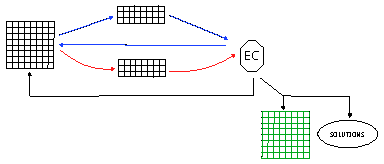
\includegraphics[width=0.75\textwidth]{partial_loading_mech.pdf}
        \label{fig:partial_loading_mech}
        \caption{The diagram tries to convey the idea that the EC function 
        is called to examine a portion of the matrix A (red arrows), then it needs to 
        read from the file other portions of the matrix A that are not given in input (blue arrows).}
    \end{figure}
\end{frame}

\begin{frame}{}
    \begin{figure}
        \centering
        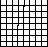
\includegraphics[width=0.45\textwidth]{grid_black.pdf}
        % \caption{}
        \label{fig:grid_black}
    \end{figure}
\end{frame}

\begin{frame}{}
    \begin{table}
        \centering
        \begin{tabular}{|c|c|}
            \hline
            Offset & Reading offset \\
            \hline
            0 & 0 \\
            \hline
        \end{tabular}
    \end{table}
    \begin{figure}
        \centering
        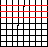
\includegraphics[width=0.45\textwidth]{grid_3r_1.pdf}
        % \caption{}
        \label{fig:grid_3r_1}
    \end{figure}
\end{frame}

\begin{frame}{}
    \begin{table}
        \centering
        \begin{tabular}{|c|c|}
            \hline
            Offset & Reading offset \\
            \hline
            0 & 0 \\
            \hline
        \end{tabular}
    \end{table}
    \begin{figure}
        \centering
        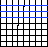
\includegraphics[width=0.45\textwidth]{grid_3r_1_ro_1.pdf}
        % \caption{}
        \label{fig:grid_3r_1_ro_1}
    \end{figure}
\end{frame}

\begin{frame}{}
    \begin{table}
        \centering
        \begin{tabular}{|c|c|}
            \hline
            Offset & Reading offset \\
            \hline
            3 & 0 \\
            \hline
        \end{tabular}
    \end{table}
    \begin{figure}
        \centering
        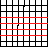
\includegraphics[width=0.45\textwidth]{grid_3r_2.pdf}
        % \caption{}
        \label{fig:grid_3r_2}
    \end{figure}
\end{frame}

\begin{frame}{}
    \begin{table}
        \centering
        \begin{tabular}{|c|c|}
            \hline
            Offset & Reading offset \\
            \hline
            3 & 0 \\
            \hline
        \end{tabular}
    \end{table}
    \begin{figure}
        \centering
        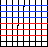
\includegraphics[width=0.45\textwidth]{grid_3r_2_ro_1.pdf}
        % \caption{}
        \label{fig:grid_3r_2_ro_1}
    \end{figure}
\end{frame}

\begin{frame}{}
    \begin{table}
        \centering
        \begin{tabular}{|c|c|}
            \hline
            Offset & Reading offset \\
            \hline
            3 & 3 \\
            \hline
        \end{tabular}
    \end{table}
    \begin{figure}
        \centering
        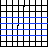
\includegraphics[width=0.45\textwidth]{grid_3r_2_ro_2.pdf}
        % \caption{}
        \label{fig:grid_3r_2_ro_2}
    \end{figure}
\end{frame}

\begin{frame}{}
    \begin{table}
        \centering
        \begin{tabular}{|c|c|}
            \hline
            Offset & Reading offset \\
            \hline
            6 & 0 \\
            \hline
        \end{tabular}
    \end{table}
    \begin{figure}
        \centering
        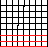
\includegraphics[width=0.45\textwidth]{grid_3r_3.pdf}
        % \caption{}
        \label{fig:grid_3r_3}
    \end{figure}
\end{frame}

\begin{frame}{}
    \begin{table}
        \centering
        \begin{tabular}{|c|c|}
            \hline
            Offset & Reading offset \\
            \hline
            6 & 0 \\
            \hline
        \end{tabular}
    \end{table}
    \begin{figure}
        \centering
        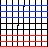
\includegraphics[width=0.45\textwidth]{grid_3r_3_ro_1.pdf}
        % \caption{}
        \label{fig:grid_3r_3_ro_1}
    \end{figure}
\end{frame}

\begin{frame}{}
    \begin{table}
        \centering
        \begin{tabular}{|c|c|}
            \hline
            Offset & Reading offset \\
            \hline
            6 & 3 \\
            \hline
        \end{tabular}
    \end{table}
    \begin{figure}
        \centering
        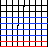
\includegraphics[width=0.45\textwidth]{grid_3r_3_ro_2.pdf}
        % \caption{}
        \label{fig:grid_3r_3_ro_2}
    \end{figure}
\end{frame}

\begin{frame}{}
    \begin{table}
        \centering
        \begin{tabular}{|c|c|}
            \hline
            Offset & Reading offset \\
            \hline
            6 & 6 \\
            \hline
        \end{tabular}
    \end{table}
    \begin{figure}
        \centering
        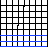
\includegraphics[width=0.45\textwidth]{grid_3r_3_ro_3.pdf}
        % \caption{}
        \label{fig:grid_3r_3_ro_3}
    \end{figure}
\end{frame}


\begin{frame}{Sudoku \footnote[frame]{The following content is 
    taken from \url{http://www.ams.org/publicoutreach/feature-column/fcarc-kanoodle}}}
    Any instance of the sudoku problem can be mapped to an instance of the exact cover problem.
    Independently of the size of the sudoku grid, which we call $N$ (where $N$ is the number
    of rows, the number of columns, the number of boxes and the number of possible
    elements to put in a cell), the exact cover problem will have 4 sets of constraints:
    \begin{enumerate}
        \item every cell has exactly one of the $N$ possible elements;
        \item every row has exactly one of the $N$ possible elements in each of its $N$ cells;
        \item every column has exactly one of the $N$ possible elements in each of its $N$ cells;
        \item every $N\times N$ box has exactly one of the $N$ possible elements in each of its $N$ cells.
    \end{enumerate}
\end{frame}

\begin{frame}
    % \scriptsize
    Each of these constraints maps to $N^2$ columns of the matrix $A$, that is to say,
    every set of the exact cover problem has $4\cdot N^2$ elements.
    The number of sets of the exact cover problem is $N^3$, where $N^2$ is the number of cells
    and $N$ is the number of possible elements to put in a cell. \\
    This is how a 1 is mapped in a row of $A$, where \\ 
    $r,c,n \in \{0,\dots,N-1\}$, $i \in \{0,\dots,4\cdot N^2-1\}$, \\
    $r$ is the row, \\
    $c$ is the column, \\
    $n$ is the element, \\
    $i$ is the index of the column of $A$:
\end{frame}
\begin{frame}    
    \begin{enumerate}
        \item a 1 in the $i$-th cell from the first $N^2$ cells of a row of $A$ (not to be confused
        with a cell of the sudoku) means that
        the [$r$-th row, $c$-th column] cell of the sudoku grid has been filled with an element, without specifying which one,
        where $i = r\cdot N + c$;
        \item a 1 in the $i$-th cell from the second $N^2$ cells of a row of $A$ means that
        the $r$-th row has been filled with the $n$-th element, where $i = N^2 + r\cdot N + n$;
        \item a 1 in the $i$-th cell from the third $N^2$ cells of a row of $A$ means that
        the $c$-th column has been filled with the $n$-th element, 
        where $i = 2\cdot N^2 + c\cdot N + n$;
        \item a 1 in the $i$-th cell from the fourth $N^2$ cells of a row of $A$ means that
        the $\big[\left\lfloor\frac{r}{\sqrt{N}}\right\rfloor$, $\left\lfloor\frac{c}{\sqrt{N}}\right\rfloor\big]$ box has been filled with the $n$-th element
        (in a $4\times 4$ sudoku the possible boxes are [0,0] (top left), 
        [0,1] (top right), [1,0] (bottom left), [1,1] (bottom right)),
        % floor(r/N^2) in latex is 
        where $i = 3\cdot N^2 + \left(\left\lfloor\frac{r}{\sqrt{N}}\right\rfloor \sqrt{N}
        + \left\lfloor\frac{c}{\sqrt{N}}\right\rfloor\right)\cdot N + n$.
    \end{enumerate}
\end{frame}
\begin{frame}{}
    In a sudoku problem there always are some numbers already written in the grid,
    the presence of more numbers makes the problem easier to solve, this reflects on the 
    exact cover problem being easier to solve, the way it becomes easier to solve is that
    the number of sets to explore decreases. One possibility is to simply remove the 
    sets that correspond to the cells that already have a number written into them but,
    in order to be able to write an algorithm that maps from the solution to the exact cover problem 
    back to the solution to the sudoku, it is easier to keep empty sets (all 0s rows),
    we can do this because our algorithm ignores the only 0s rows, so the search tree will be pruned anyway
    during the execution of the algorithm.
\end{frame}

\begin{frame}{}
    % CODE TO TRANSLATE INTO PSEUDOCODE
    % def sudoku_to_exact_cover(sudoku, N):
    % constraints = 4  # Cell, Row, Column, Box
    % cover_matrix = [[0] * (N * N * constraints) for _ in range(N * N * N)]
    % divider = int(N ** 0.5)
    % for r in range(N):
    %     for c in range(N):
    %         for n in range(N):
    %             # Calculate row index for cover_matrix
    %             idx = (r * N + c) * N + n
                
    %             # Cell constraint - first N^2 columns
    %             cover_matrix[idx][r * N + c] = 1

    %             # Row constraint - second N^2 columns
    %             cover_matrix[idx][N * N + r * N + n] = 1

    %             # Column constraint - third N^2 columns
    %             cover_matrix[idx][2 * N * N + c * N + n] = 1

    %             # Box constraint - last N^2 columns
    %             box_row = r // divider
    %             box_col = c // divider
    %             box_num = box_row * divider + box_col  # This has changed from 3 to 2 for 4x4 Sudoku
    %             cover_matrix[idx][3 * N * N + box_num * N + n] = 1
                
    % # Prune rows that conflict with given Sudoku puzzle
    % # by setting them to all zeros

    % rows_to_remove = []
    % for r in range(N):
    %     for c in range(N):
    %         num = sudoku[r * N + c]-1
    %         if num+1:
    %             start_idx = (r * N + c) * N
    %             for i in range(N):
    %                 if i != num:
    %                     rows_to_remove.append(start_idx + i)


    % for idx in sorted(rows_to_remove):
    %     # Setting the row to all zeros
    %     cover_matrix[idx] = [0] * (N * N * constraints)
                
    % return cover_matrix
    \
    \begin{algorithmic}
        \Function{SudokuToExactCover}{$sudoku[], N$}
            \Comment{$sudoku$ is an array of length $N^2$ containing the numbers written in the sudoku grid}
            \State $nConstraints \gets 4$
            \State $coverMatrix \gets \Call{zeros}{N^3, N^2\cdot nConstraints}$
            \State \Call{FillA}{coverMatrix, N}
            % \For{$r \gets 0$ to $N-1$}
            %     \For{$c \gets 0$ to $N-1$}
            %         \For{$n \gets 0$ to $N-1$}
            %             \State $idx \gets (r\cdot N + c)\cdot N + n$
            %             \State $coverMatrix[idx][r\cdot N + c] \gets 1$
            %             \State $coverMatrix[idx][N^2 + r\cdot N + n] \gets 1$
            %             \State $coverMatrix[idx][2\cdot N^2 + c\cdot N + n] \gets 1$
            %             \State $boxRow \gets \lfloor r / \sqrt{N} \rfloor$
            %             \State $boxCol \gets \lfloor c / \sqrt{N} \rfloor$
            %             \State $boxNum \gets boxRow\cdot \sqrt{N} + boxCol$
            %             \State $coverMatrix[idx][3\cdot N^2 + boxNum\cdot N + n] \gets 1$
            %         \EndFor
            %     \EndFor
            % \EndFor
            \State $rowsToRemove \gets \Call{set}{\emptyset}$
            \State \Call{PruneRows}{$rowsToRemove$, $sudoku$, $N$}
            % \For{$r \gets 0$ to $N-1$}
            %     \For{$c \gets 0$ to $N-1$}
            %         \State $symbol \gets sudoku[r\cdot N + c] - 1$ \Comment{Numbers in a sudoku 
            %         usually start from 1, but in the matrix A they start from 0}
            %         \If{$num$ is not \textbf{NULL}} \Comment{\textbf{NULL} means that the cell is empty}
            %             \State $startIdx \gets (r\cdot N + c)\cdot N$
            %             \For{$i \gets 0$ to $N-1$}
            %                 \If{$i \neq num$}
            %                     \State $rowsToRemove \gets rowsToRemove \cup \{startIdx + i\}$
            %                 \EndIf
            %             \EndFor
            %         \EndIf
            %     \EndFor
            % \EndFor
            \For{$idx \in rowsToRemove$}
                \State $coverMatrix[idx] \gets \Call{zeros}{N^2\cdot nConstraints}$
            \EndFor
            \State \Return $coverMatrix$
        \EndFunction
    \end{algorithmic}
\end{frame}

\begin{frame}{}
    \begin{algorithmic}
        \Function{FillA}{$coverMatrix$, $N$}
            \For{$r \gets 0$ to $N-1$}
                \For{$c \gets 0$ to $N-1$}
                    \For{$n \gets 0$ to $N-1$}
                        \State $idx \gets (r\cdot N + c)\cdot N + n$
                        \State $coverMatrix[idx][r\cdot N + c] \gets 1$
                        \State $coverMatrix[idx][N^2 + r\cdot N + n] \gets 1$
                        \State $coverMatrix[idx][2\cdot N^2 + c\cdot N + n] \gets 1$
                        \State $boxRow \gets \lfloor r / \sqrt{N} \rfloor$
                        \State $boxCol \gets \lfloor c / \sqrt{N} \rfloor$
                        \State $b \gets boxRow\cdot \sqrt{N} + boxCol$
                        \State $coverMatrix[idx][3\cdot N^2 + b\cdot N + n] \gets 1$
                    \EndFor
                \EndFor
            \EndFor
        \EndFunction
    \end{algorithmic}
\end{frame}

\begin{frame}{}
    \begin{algorithmic}
        \Function{PruneRows}{$rowsToRemove$, $sudoku$, $N$}
            \For{$r \gets 0$ to $N-1$}
                \For{$c \gets 0$ to $N-1$}
                    \State $symbol \gets sudoku[r\cdot N + c] - 1$ \Comment{Numbers in a sudoku 
                    usually start from 1, but in the matrix A they start from 0}
                    \If{$num$ is not \textbf{NULL}}
                        \State $startIdx \gets (r\cdot N + c)\cdot N$
                        \For{$i \gets 0$ to $N-1$}
                            \If{$i \neq num$}
                                \State $rowsToRemove \gets rowsToRemove \cup \{startIdx + i\}$
                            \EndIf
                        \EndFor
                    \EndIf
                \EndFor
            \EndFor
        \EndFunction
    \end{algorithmic}
\end{frame}

\begin{frame}{}
    % def exact_cover_solution_to_sudoku(partition, N):
    % solution = [[0] * N for _ in range(N)]
    
    % for idx in partition:
    %     r, c, n = idx // (N * N), (idx // N) % N, (idx % N) + 1
    %     solution[r][c] = n
        
    % return solution
    \begin{algorithmic}
        \Function{ExactCoverSolutionToSudoku}{$ecSolution[], N$}
            \State $sudokuSolution \gets \Call{zeros}{N, N}$
            \For{$idx \in ecSolution$}
                \State $r \gets \left\lfloor \frac{idx}{(N^2)} \right\rfloor$
                \State $c \gets \left\lfloor (\frac{idx}{N}) \mod N \right\rfloor$
                \State $n \gets (idx \mod N) + 1$
                \State $sudokuSolution[r][c] \gets n$
            \EndFor
            \State \Return $sudokuSolution$
        \EndFunction
    \end{algorithmic}
\end{frame}

\begin{frame}{Generating Exact Cover problems}
    Having a module that generates exact cover problems given the 
    number of sets and the cardinality of the domain of the sets is
    useful for testing purposes.
    The idea of my choice is to ensure
    that every generated problem has at least a solution (that is, at least a set 
    of sets that cover all the elements of the domain),
    this is done by setting randomly $M$ rows of the matrix $A$ to 
    the canonical base of $\mathbb{R}^M$.
    The precondition is that $N \geq M$.
    The rows of the matrix $A$ that are not set to the canonical base
    are filled randomly, each of their $M$ cells is set to 1 or 0 with
    a custom probability, the default one is $p=0.5$.
\end{frame}

\begin{frame}{}
    \begin{algorithmic}
        \Function{GenerateExactCover}{$N$, $M$}
            \If {$N < M$}
                \State \Return \textbf{NULL}
            \EndIf
            \State $A \gets \Call{zeros}{N, M}$
            % # Choose a solution
            % selected_rows = random.sample(range(N), M)
            % for i, row in enumerate(selected_rows):
            %     matrix[row][i] = 1            
            \State $idxCanonicalBase[] \gets \Call{RandomSample}{\{0,\dots,N-1\}, M}$ 
            \Comment{Sample from $\{0,\dots,N-1\}$ without replacement for $M$ times}
            \For{$i \gets 0$ to $M-1$}
                \State $A[idxCanonicalBase[i]][i] \gets 1$
            \EndFor

            % # Add noise to remaining rows
            % for i in range(N):
            %     if i not in selected_rows:
            %         for j in range(M):
            %             matrix[i][j] = random.choice([0, 1])  
            \For{$i \gets 0$ to $N-1$}
                \If{$i \notin idxCanonicalBase$}
                    \For{$j \gets 0$ to $M-1$}
                        \State $A[i][j] \gets \Call{RandomChoice}{\{0,1\}}$
                    \EndFor
                \EndIf
            \EndFor
            \State \Return $A$
        \EndFunction
    \end{algorithmic}
\end{frame}          

\end{document}